\def\thelstlisting{}

%不需要区分奇偶页的请使用下面一行
\documentclass[a4paper,AutoFakeBold,oneside,12pt]{book}
%需要区分奇偶页的(即每一章第一页一定在奇数页上)请使用下面一行
%\documentclass[a4paper,AutoFakeBold,openright,12pt]{book}
\usepackage{BUPTthesisbachelor}
\usepackage{setspace}

%\lstdefinestyle{sharpc}{language=[Sharp]C, frame=lrtb, rulecolor=\color{blue!80!black}}


%%%%%%%%%%%%%%%%%%%%%%%%% Begin Documents %%%%%%%%%%%%%%%%%%%%%%%%%%
\begin{document}

% 封面
\blankmatter

\includepdf[pages=-]{docs/cover.pdf}

% 任务书
% \blankmatter
% 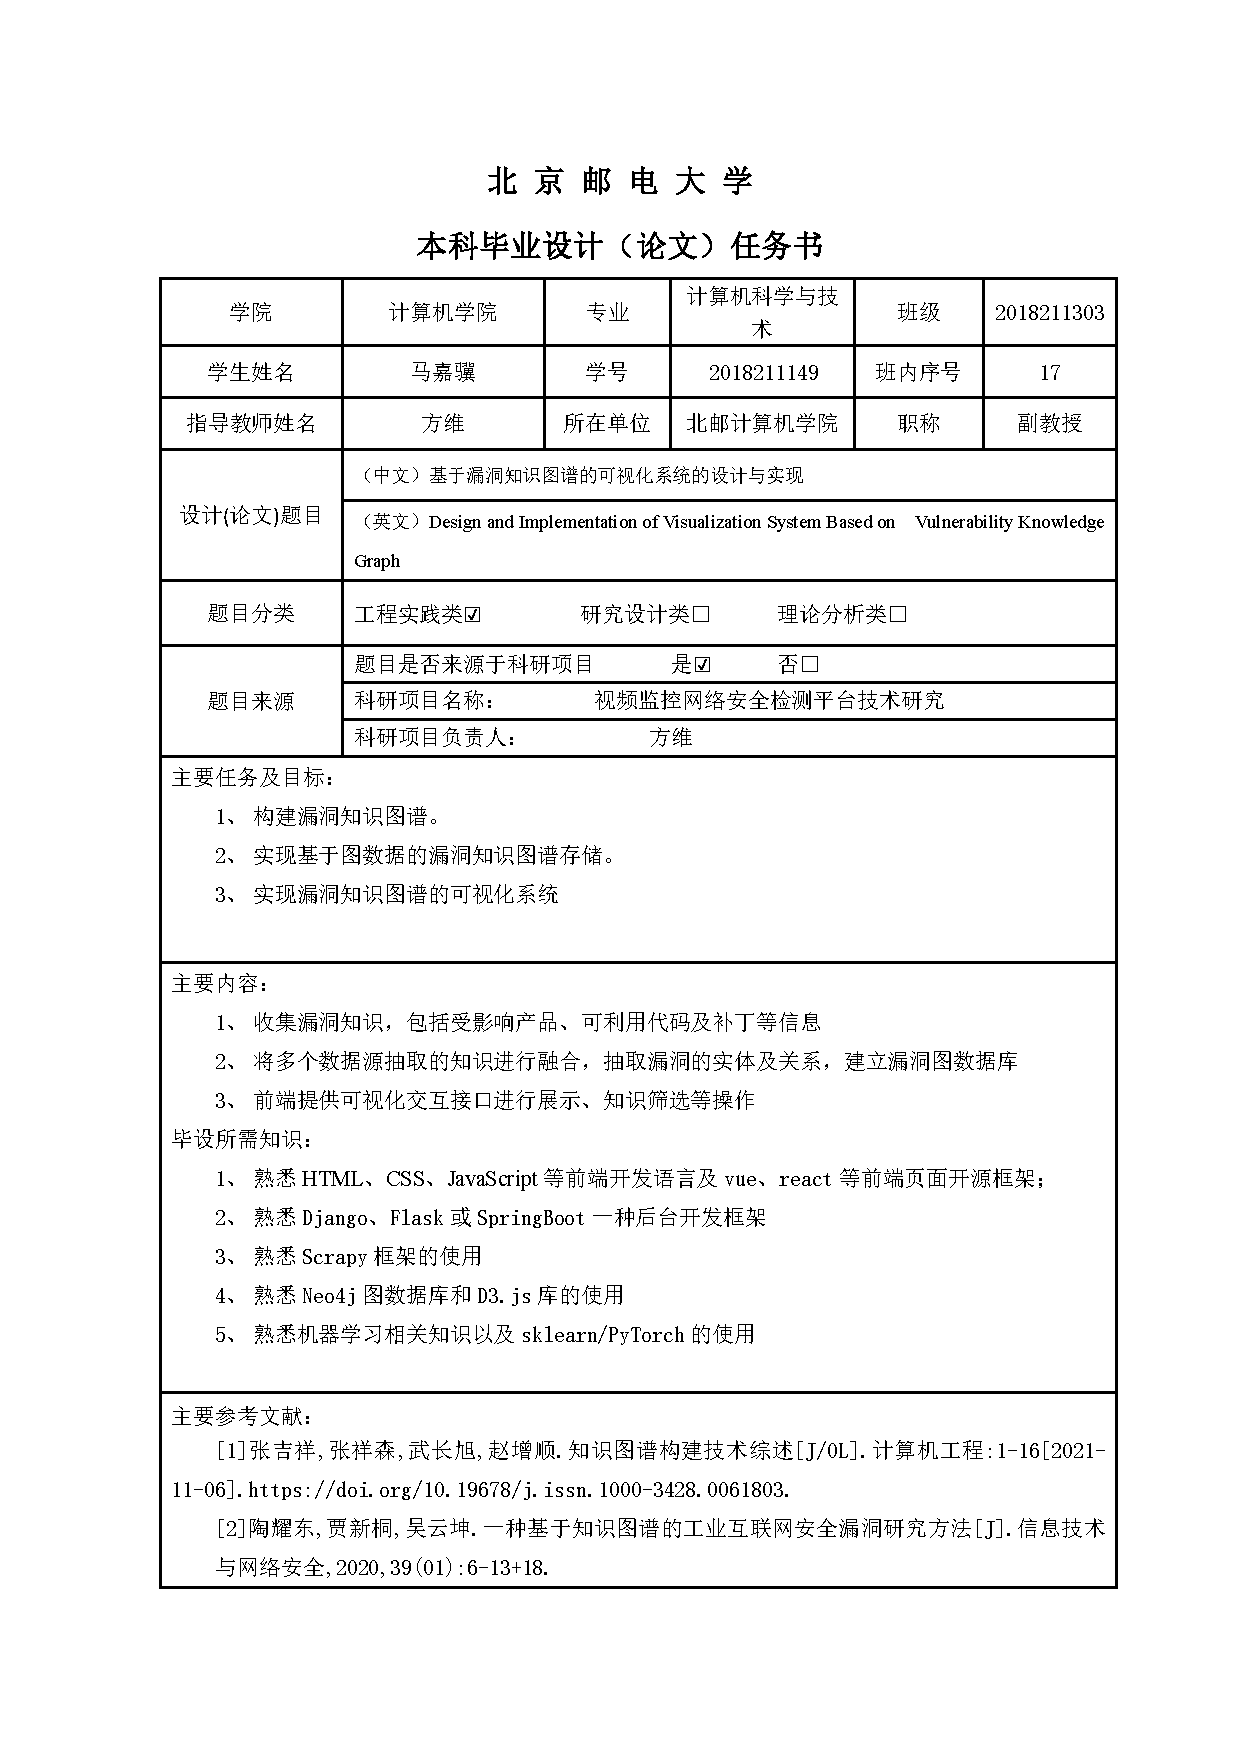
\includepdf[pages=-]{docs/task.pdf}

% 成绩评定表
% \blankmatter
% 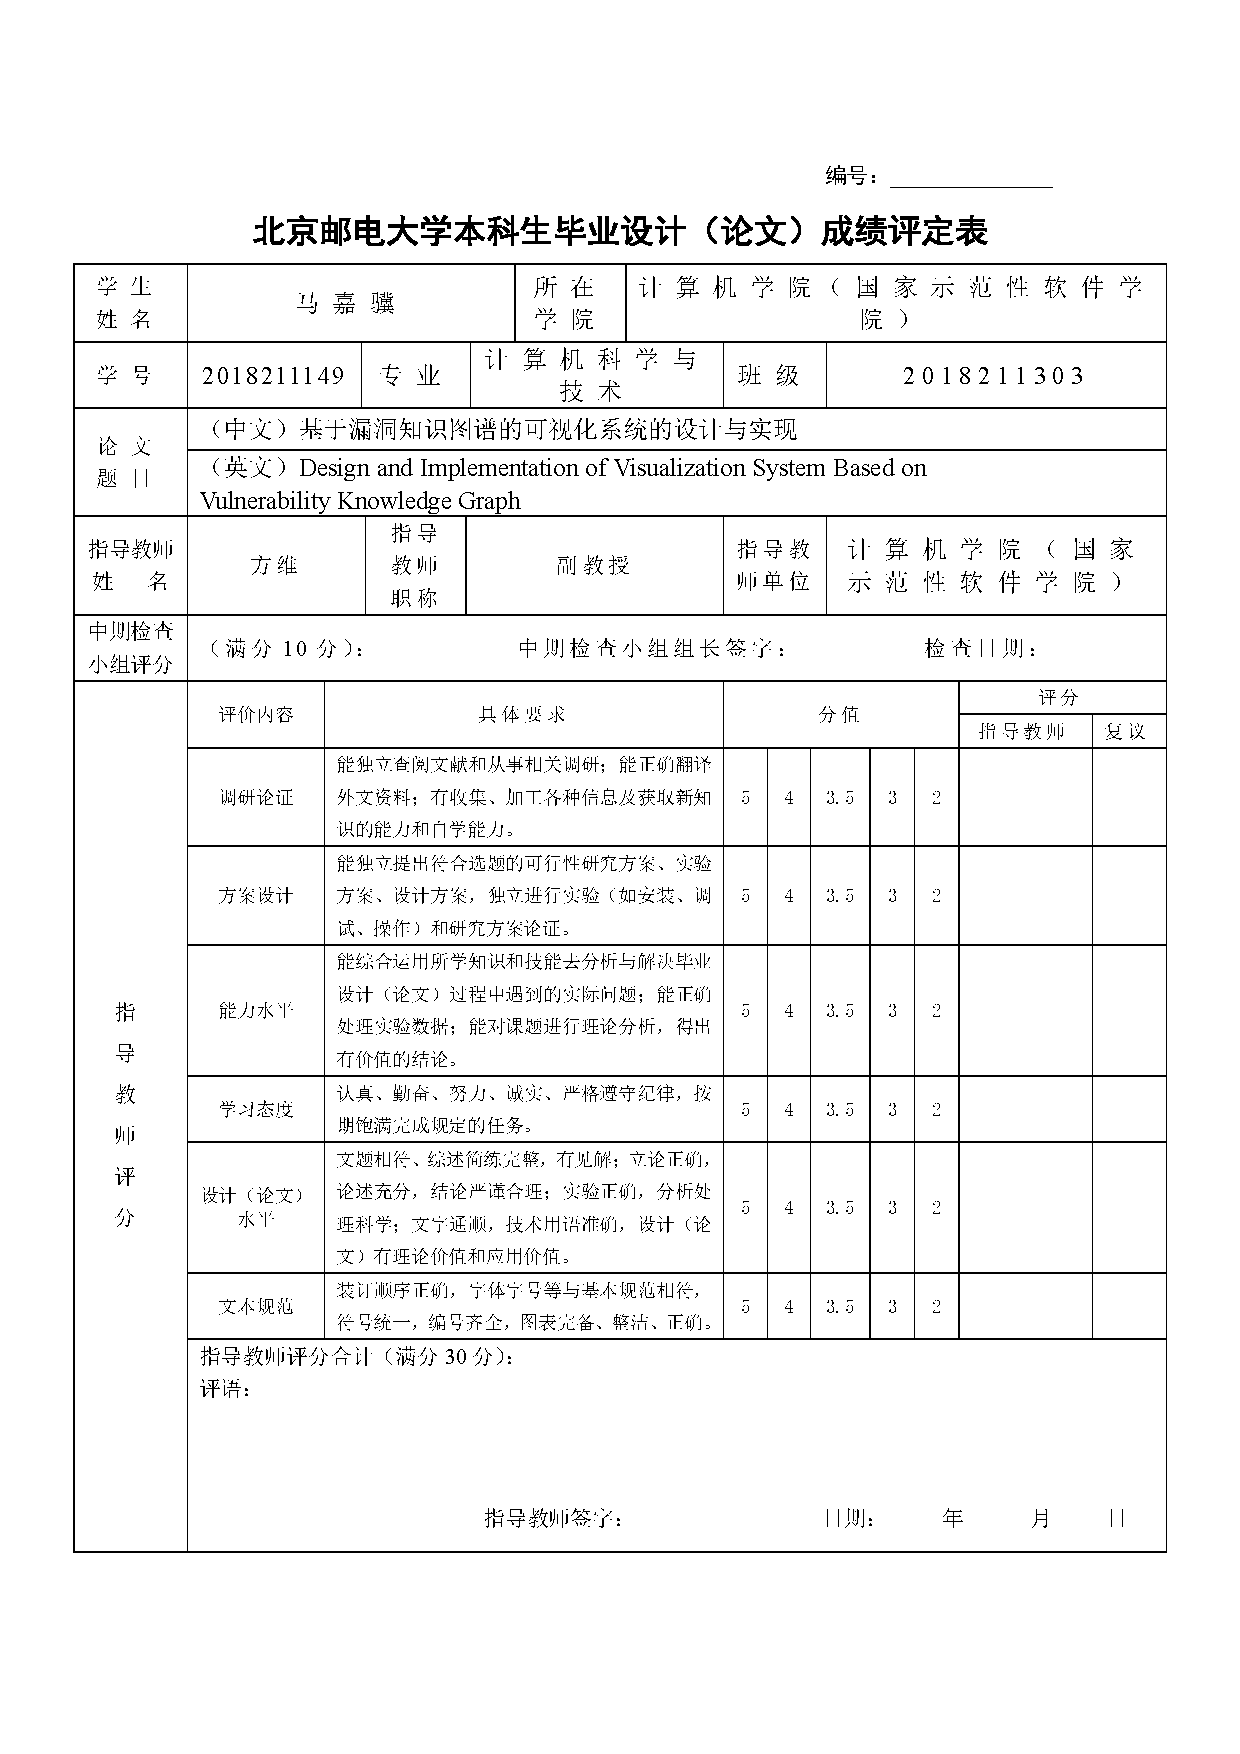
\includepdf[pages=-]{docs/scoreTable.pdf}

% 诚信声明
% \blankmatter
% 
\includepdf[pages=-]{docs/statement.pdf}

%%%%%%%%%%%%%%%%%%%%%%%%%%%%%%%%%%%%%%%%%%%%%%%%%%%%%%%%%%%%%%%%%%%%
%                                                                  %
%   Copyright (c) 2010 - 2011 Caspar Zhang <casparant@gmail.com>   %
%                                                                  %
%   This copyrighted material is made available to anyone wishing  %
%   to use, modify, copy, or redistribute it subject to the terms  %
%   and conditions of the GNU General Public License version 2.    %
%                                                                  %
%   This program is distributed in the hope that it will be        %
%   useful, but WITHOUT ANY WARRANTY; without even the implied     %
%   warranty of MERCHANTABILITY or FITNESS FOR A PARTICULAR        %
%   PURPOSE. See the GNU General Public License for more details.  %
%                                                                  %
%   You should have received a copy of the GNU General Public      %
%   License along with this program; if not, write to the Free     %
%   Software Foundation, Inc., 51 Franklin Street, Fifth Floor,    %
%   Boston, MA 02110-1301, USA.                                    %
%                                                                  %
%%%%%%%%%%%%%%%%%%%%%%%%%%%%%%%%%%%%%%%%%%%%%%%%%%%%%%%%%%%%%%%%%%%%

% 你只需要修改下面几行就可以完成大部分内容的填写,
% 这要求你具有一定的LaTeX基础,但是如果你足够聪明,
% 不具有LaTeX基础也可以完成。

% 论文中文题目
\def\thesistitle{基于知识图谱的可视化系统的设计与实现}

% 论文英文题目
%提示:英文摘要页的标题注意格式要求。
\def\thesistitleen{Design and Implementation of Visualization System Based on Vulnerability Knowledge Graph}

% Thank Words
\def\thankwords{

感谢。

}
    % Main items 
%%%%%%%%%%%%%%%%%%%%%%%%%%%%%%%%%%%%%%%%%%%%%%%%%%%%%%%%%%%%%%%%%%%%
%                                                                  %
%   Copyright (c) 2010 - 2011 Caspar Zhang <casparant@gmail.com>   %
%                                                                  %
%   This copyrighted material is made available to anyone wishing  %
%   to use, modify, copy, or redistribute it subject to the terms  %
%   and conditions of the GNU General Public License version 2.    %
%                                                                  %
%   This program is distributed in the hope that it will be        %
%   useful, but WITHOUT ANY WARRANTY; without even the implied     %
%   warranty of MERCHANTABILITY or FITNESS FOR A PARTICULAR        %
%   PURPOSE. See the GNU General Public License for more details.  %
%                                                                  %
%   You should have received a copy of the GNU General Public      %
%   License along with this program; if not, write to the Free     %
%   Software Foundation, Inc., 51 Franklin Street, Fifth Floor,    %
%   Boston, MA 02110-1301, USA.                                    %
%                                                                  %
%%%%%%%%%%%%%%%%%%%%%%%%%%%%%%%%%%%%%%%%%%%%%%%%%%%%%%%%%%%%%%%%%%%%

% 你只需要修改下面内容就可以完成中英文摘要,
% 这要求你具有一定的LaTeX基础,但是还是那句话,
% 如果你足够聪明,不具有LaTeX基础也可以完成。

% 中文摘要
\def\abstractzh{
%从这里开始写你的摘要,分段需要空一行。
这是中文摘要的部分。

它可以拥有多段。
这是中文摘要的部分。

它可以拥有多段。

如果你写的太长,甚至可以到第二页。
%摘要结束
}

% 中文关键字 
% TODO: 改成可变长度的
\def\abszhkeyone{北京邮电大学}
\def\abszhkeytwo{本科生}
\def\abszhkeythree{毕业设计}
\def\abszhkeyfour{模板}
\def\abszhkeyfive{示例}

% ABSTRACT
\def\abstracten{
%Your abstract here, to make a new paragraph, give an extra blank line please.
This is ABSTRACT.

You can write more than one paragraph here.

If your abstract is too long, it will take up more pages. 
%Abstract done
}

% Key Words 
% TODO: 改成可变长度的
\def\absenkeyone{BUPT}
\def\absenkeytwo{undergraduate}
\def\absenkeythree{thesis}
\def\absenkeyfour{template}
\def\absenkeyfive{example}


  % Abstract
\fancypagestyle{plain}{\pagestyle{frontmatter}}
\frontmatter\tableofcontents % Content


% 正文
\newpage\mainmatter
\fancypagestyle{plain}{\pagestyle{mainmatter}}
%\let\cleardoublepagebak=\cleardoublepage
%\let\cleardoublepage\relax % Make new chapter stay on old page

%%%%%%%%%%%%%%%%%%%%%%%%%%%%% Main Area %%%%%%%%%%%%%%%%%%%%%%%%%%%%
\sloppy

\chapter{绪论}

\section{项目背景及意义}

\subsection{选题背景}
% 这段先放着
% \begin{definition}
% 	计算机安全、互联网信息安全,或信息安全技术意指对计算机系统及计算机网络施加保护手段,以使其不受信息披露、信息盗取、软硬件或电子信息损坏等危害,使其\cite{wilson_fundamental_2014}
% \end{definition}
% 这段先放着

近年来,随着互联网产业迅速发展,互联网安全漏洞问题的显著性也急剧增加。根据公共漏洞和暴露\footnote{Common Vulnerabilities and Exposures, CVE}、国家信息安全漏洞库\footnote{China National Vulnerability Database of Information Security, CNNVD}等业内权威的漏洞数据档案库的数据\cite{download_cve_list}\cite{nvd_cpe_statistics},自 1999 年 CVE 漏洞库首次披露安全漏洞以来,互联网安全漏洞年新增数量呈增长趋势。2019 年全年,新增漏洞两万余个;2020 年全年,新增漏洞三万五千余个。随着现代软件系统复杂度提升、互联网加速漏洞信息传播,对攻击者而言,不仅漏洞攻击的学习成本和实施难度下降,其可以利用的漏洞数量也明显增多\cite{vuldb_stats};对企业与开发者而言,随着开源化逐渐成为一种潮流趋势,各类计算机软硬件与互联网产品对开源项目的依赖性随之提高。正如近期 Java Log4j 日志组件漏洞造成全球互联网范围的大规模信息安全问题,计算机与互联网产业在快速发展的同时,也面临着与日俱增的信息安全挑战。

\subsection{国内外研究现状}

网络安全意指一组用于保护计算机、网络、程序与数据免受攻击、未授权访问、篡改、破坏的技术与步骤\cite{aftergood_cybersecurity_2017}。提供详实可靠的漏洞信息可以有效地帮助互联网安全研究人员进行网络安全研究,以应对可能存在的攻击和利用。针对互联网漏洞数据,主要分为公开数据库与商业项目。

\subsubsection{公开数据库}

如 cve.mitre.org、nvd.nist.gov、vuldb.com 等。

\begin{itemize}
	\item 优势:
	      \begin{itemize}
		      \item 数据更新及时,CVE 与 CPE 为官方数据源
		      \item 开放数据库,人人可获取
	      \end{itemize}
	\item 劣势:
	      \begin{itemize}
		      \item 无知识图谱,不具备可视化功能,仅提供 JSON 或 CSV 文件格式存储关系型数据
		      \item 按照 CVE ID 索引漏洞信息,难以发现漏洞之间联系
		      \item 信息分散在多个站点,难以整合,为研究人员带来不便
	      \end{itemize}
\end{itemize}

\subsubsection{商业项目}

如百度安全知识图谱\footnote{https://anquan.baidu.com/product/skg}、绿盟安全知识图谱\footnote{https://www.nsfocus.com.cn/html/2022/209{\_}0510/163.html}等。

\begin{itemize}
	\item 优势:
	      \begin{itemize}
		      \item 成熟的企业级解决方案与技术支持
		      \item 具备知识图谱的可视化功能
	      \end{itemize}
	\item 劣势:
	      \begin{itemize}
		      \item 数据不开放,对安全研究人员及软件开发者意义有限
		      \item 价格高昂
	      \end{itemize}
\end{itemize}

\subsection{项目意义}

本课题针对上述问题,提出一种漏洞知识图谱可视化系统。基于爬虫抽取、知识图谱、图数据库、可视化前端等技术,对多种数据源的互联网公开漏洞数据,包括漏洞描述及风险评估、受影响资产、可利用代码及补丁等信息进行收集与分析,通过对异构数据源抽取的数据进行实体构建、关系构建、关系融合等处理,在图数据库中建立漏洞本体信息及其之间的关联信息,从而形成具有一定知识结构的知识图谱。基于该漏洞知识图谱,搭建基于 B/S 架构的可视化系统,提供易于使用的接口、用户友好的 UI 界面呈现漏洞知识图谱信息、进行创建统计图表、知识筛选等操作。

本系统采用自动化的方式,实现对漏洞信息的持续收集与整理,极大节省了人力资源的消耗。结合抽取关键信息建立互联网信息安全本体、对漏洞间关联性进行分析、构建漏洞知识图谱,将分散的漏洞信息转化为相互联系的图结构,本系统将为开发者提供项目依赖安全性参考、为计算机信息安全研究人员提供逻辑清晰、直观易于理解的统计数据与服务支撑。

本系统作为自由软件\cite{libre_software}发布,使用 GPL-3.0\cite{gpl_v3} 许可证授权,自由与开放促进构建更高效安全的互联网环境。

\section{开发目标}

\begin{itemize}
	\item 设计并实现对异构公开互联网信息漏洞数据源的信息采集子系统。
	\item 设计并实现基于规则的漏洞知识图谱构建子系统。
	\item 设计并实现基于图数据库的漏洞知识图谱持久化子系统。
	\item 设计并实现基于上述漏洞知识图谱的后端服务子系统,提供 RESTful API 访问点。
	\item 设计并实现基于 Web 服务的漏洞知识图谱可视化子系统,具备独立前端。
	\item 对上述系统进行系统测试、排错、功能扩展、性能优化,编写文档记录。
\end{itemize}

\section{软件工程方法}

由于本项目为单人完成,且系统整体结构较为复杂,故采用原型开发与敏捷开发\cite{manifesto_agile_dev}相结合的方式,先开发最简可行产品\cite{minimum_viable_product}(Minimum Viable Product, MVP)验证核心概念,在此基础上不断细化细节、完善代码、扩展功能。同时,因为单人项目难以在前期进行完善的需求分析与系统设计,采用敏捷开发的方式可以增强灵活性。

例如,本项目立项初期技术选型,计划使用较为成熟的 Java Springboot 框架搭建后端服务。在之后的开发中发现,由于该项目对数据库操作需求较高,其他子系统使用 Python 而后端使用 Springboot 意味着需要使用 Python 和 Java 分别编写两套代码用于控制数据库驱动,增加无意义的项目复杂度、拖慢开发进度。得益于敏捷开发思想``响应变化高于遵循计划''等方针,本项目在知识图谱构建子系统的原型开发完成时即更改后端使用 Python Flask 进行开发,从而保证软件质量的同时提升开发效率。

\section{授权与许可证}

本系统作为自由软件\cite{libre_software}发布,使用 GPL-3.0\cite{gpl_v3} 许可证授权,全部代码在 \href{https://github.com/RiddMa/KnowledgeGraph-Visualization}{GitHub}\footnote{https://github.com/RiddMa/KnowledgeGraph-Visualization} 开源。

\chapter{相关技术介绍}

根据系统开发目标,可将系统层次结构从信息处理逻辑上分为三个层次:用于持久化存储信息的持久化层,用于对信息进行采集、处理、传输的逻辑层,用于面向用户展示信息的表示层;从功能上分为五类技术:数据采集技术、知识图谱构建技术、持久化子技术、后端技术、前端技术。本章从功能的五个方面分别介绍本项目使用的相关技术。

\section{数据采集技术}

采用的技术或工具:Scrapy、Pandas

\subsection{Scrapy}

Scrapy\footnote{https://scrapy.org/} 是自由且开源的协作式网络爬虫 Python 框架,用于从网站或 API 中提取需要的数据。Scrapy 基于 Twisted,具有快速、易用、可扩展等特性,主要优点是架构清晰、模块间的耦合程度低、通过 Middleware 钩子框架能灵活完成各种需求。Scrapy 项目围绕 Spider 类构建,并具有 Item Pipelines、Downloader、Scheduler 等多个模块,这些模块通过内置的 Scrapy Engine 进行管理与调度。Scrapy 设计理念遵循``一次且仅一次''(Once and only once, OAOO)原则,主张为每个爬虫任务只需要编写一个自包含(self-contained)的 Spider 类,没有更多,没有更少。

相较于 urllib 或 Python Requests 等基础的库,Scrapy 提供任务日志、错误重试、并发控制,具备更灵活完善的机制以应对大型爬虫任务。而相较于 Selenium、Puppeteer、Playwright 等基于无头浏览器(Headless Browser)实现的爬虫功能,Scrapy 基于事件驱动的网络编程框架 Twisted,仅爬取 HTML 文档,默认不提供执行网页中的 JavaScript 代码功能,因此 CPU 与内存开销相较无头浏览器显著减小,是最适合本系统大量数据爬取需求的框架。

\subsection{Pandas}

Pandas\footnote{https://pandas.pydata.org/} 是适用于 Python 语言的数据操纵与分析库,是使用 BSD 许可证授权发行的自由且开源的软件,尤其擅长数值表格与时间序列的数据结构和运算操作。

本数据采集子系统将从 cve.mitre.org 爬取其提供的包含全部 cve id 信息的 csv 文件,其中包含数十万条 cve 漏洞 id 条目。由于该 csv 文件包含表头信息及一些无效或重复的 cve id,在建立用于从异构数据源爬取项目的 cve id 索引时需要将无关信息删去。该 csv 文件体积较大(约数百兆字节),因此使用 Pandas 提供的流式读取 csv 文件、迭代操作的方法处理此文件。

\section{知识图谱构建技术}

采用的技术或工具:基于规则的实体构建、基于规则的关系生成、Ray。实体构建与关系生成技术将在章节 \ref{知识图谱构建子系统} \nameref{知识图谱构建子系统}展开。

\subsection{知识图谱概念}

近年来,使用知识图谱表达人类知识结构受到了学术界与工业界的极大关注。知识图谱是事实、实体构成、关系和语义的结构化表达,是一种用图表示的数据结构。知识图谱存储实体结点、结点之间的关系,旨在积累并表达现实世界的知识。\cite{ji_survey_2022}

知识图谱的图结点代表被研究的实体,实体可以是现实世界的对象或抽象的概念。实体结点之间的边代表实体之间的关系,以及实体的语义描述,它们的关系具有类型和明确定义的属性。\cite{ji_survey_2022}用于存储知识图谱数据的图遵从基于图结构的数据模型,如有向的边标记图或属性图。\cite{hogan_knowledge_2022}

通常以三元组的形式表达知识图谱结构,即
$$G=(Entity_{head}, Relation, Entity_{tail})$$
$Entity_{head}$为三元组$G$的头实体,是关系的起点。$Entity_{tail}$为三元组$G$的尾实体,是关系的终点。实体表示被建模的现实的对象或抽象的概念。$Relation$则表示$Entity_{head}$到$Entity_{tail}$的语义化关系。\cite{hogan_knowledge_2022}

知识图谱在信息检索中的应用价值主要在于,它能通过推理实现概念检索,以图形化的方式,向用户展示经过分类整理的结构化知识,从而使人从人工筛选、过滤数据寻找答案的模式中解放出来。在漏洞数据库的基础上,构建漏洞知识图谱,挖掘互联网信息安全漏洞内在特性、关联关系等价值,有助于多维度、全方位地理解安全漏洞关系。

\subsection{知识图谱构建过程}

知识图谱主要包含开放知识图谱和领域知识图谱。开放知识图谱如 Wikipedia、Freebase、DBpedia 等,往往采用自底向上方法构建。而互联网信息安全漏洞知识图谱属于领域知识图谱,适宜采用自顶向下构建方法,即通过人工整理出领域知识图谱的实体及关系模型图,进行实体和关系的抽取与知识图谱的构建。在安全漏洞领域中,预先定义的实体与关系模型能极大提高知识图谱的构建质量及应用效率。\cite{zhang_survey_2021}

实体抽取:又称命名实体识别(Named Entity Recognition, NER),主要分为基于规则的方法、基于传统机器学习的方法、基于深度学习的方法\cite{zhou_survey_2020},后两者主要用于解决从自然语言文本中抽取未预定义格式信息的问题。本项目相关安全漏洞领域实体具有明确名称与格式,适宜采用基于规则的方法提取。未来系统扩展如博客、新闻等小部分自然语言数据源,可采用基于深度学习的方法如 CNN-Bi-LSTM-CRF 等模型进行命名实体识别。

关系抽取(Relationship Extraction, RE):主要分为基于传统规则和模板的方法、基于传统机器学习的方法、基于深度学习的方法\cite{zhou_survey_2020}。安全漏洞领域实体如漏洞、资产、利用等类别较少且具备明确语义关系,因此采用基于传统规则的关系抽取方法。

\subsection{Ray}

Ray\footnote{https://docs.ray.io/en/latest/} 是一个开源的通用分布式计算框架,由加州大学伯克利分校的 RISE 实验室开发。Ray 为构建分布式应用提供了一个简单、通用的 API,提供了运行机器学习工作流的 Ray ML 工具箱、运行分布式应用的 Ray Core 核心框架、部署大规模工作负载的 Ray Cluster 集群等,具有通用的分布式计算抽象以及优秀的性能。

相较传统的分布式框架(如 Hadoop、Spark 等),Ray 可直接通过 pip 进行安装,具备轻量级的特性。同时它通过共享内存实现了高效的数据存储和传输,通过全局状态存储服务实现了全局的状态维护、去中心化的高效调度、远程调用。相较基于线程的并行库  threading,Ray 通过进程级并行绕过了 Python 全局解释器锁的限制。相较轻量级的 Python 进程级并行库 multiprocessing,Ray 具备同样简单易用的接口以及更优秀的性能与机器学习框架整合能力。

本项目通过使用 Ray 框架提供的通用分布式计算能力,对上层封装具体实现;将知识图谱构建过程抽象成创建结点、创建关系、关系融合三个操作,重点优化这三个步骤的代码实现,使``数据采集子系统得到的原始数据通过知识图谱构建子系统形成知识图谱''过程得以实现并行化计算,充分利用多核心处理器的计算能力。同时,得益于 Ray 框架对本地多进程与分布式多进程的统一抽象、Ray ML 框架与深度学习模型良好的整合能力,未来可以引入深度学习模型、将系统迁移扩展至分布式计算平台。

\section{持久化技术}

采用的技术或工具:MongoDB、Neo4j

\subsection{MongoDB}

MongoDB\footnote{https://www.mongodb.com/} 是一个 C++ 语言编写的基于分布式文件存储的开源文档型数据库系统,是最受欢迎的 NoSQL 数据库。MongoDB 基于 JSON/BSON 格式的文档存储,相较传统 SQL 数据库可以表示灵活的数据结构;具备动态 DDL 能力、没有强 Schema 约束的特性使其支持开发者进行快速迭代;提供基于内存的快速数据查询,实现高并发计算性能;提供数据分片能力,分布式扩展性强。

本项目需求从异构数据源采集互联网信息安全漏洞数据,导致数据格式繁多,在项目初期规定数据所采用的 Schema 格式将大幅增加数据转换工作量,并不现实。因此,传统 SQL 关系型数据库并不适合本项目的开发需求。而 MongoDB 提供面向文档的 JSON 存储,适配互联网爬虫数据采集需求。同时,JSON 文件具备良好的序列化能力,且与本项目后端服务子系统 RESTful API 所需的 Application/JSON Response 相匹配。更进一步地,MongoDB 具有优秀的分布式能力。综上原因,采用 MongoDB 作为存储知识图谱所用原始数据的数据库。

\subsection{Neo4j}

Neo4j\footnote{https://neo4j.com/} 是一个高性能的图形数据库,是目前全球范围内最受欢迎、使用人数最多的图数据库,社区版本采用 GPL-3.0 许可证授权。其特点是将结构化数据存储在网状结构上,使得长程、广范围关系查询变得更加容易实现,Neo4j 是目前使用最多的图数据库。本项目的知识图谱构建子系统使用 Neo4j 存储图谱数据,将漏洞、资产、利用代码等实体作为结点,为结点之间添加``影响''、``具有''、``攻击''、``被攻击''、``父级''、``子级''等关系,形成知识网络图谱。

\section{后端技术}

采用的技术或工具:Flask、Advanced Python Scheduler

\subsection{Flask}

Flask\footnote{https://flask.palletsprojects.com/en/2.1.x/} 是一个使用 Python 编写的轻量级 Web 应用框架,具备微核心与高扩展性,使用 BSD 许可证授权发行。Flask 是在 Jinja2 模板引擎和 Werkzeug WSGI 工具箱的基础上构建的。Werkzeug 是一个语言网络服务器网关接口(Web Server Gateway Interface, WSGI),为请求、相应等功能实现软件对象;Jinja 是一个适用于 Python 的网页模板引擎。

本项目主要使用 Flask 框架的 WSGI 功能,构建一个 RESTful 风格的 Web API 服务,为 Vue.js 编写的前端提供与数据库的交互功能。本着``高内聚,低耦合''的设计原则,同时兼具部署简洁、外部依赖较少、用户控制灵活的优点,本基于漏洞知识图谱的可视化系统将前述数据采集子系统、知识图谱构建子系统抽象成自包含的服务,仅通过持久化层的 MongoDB 及 Neo4j 数据库进行纯数据交换,最大程度上减少模块间逻辑耦合。

由于数据采集子系统、知识图谱构建子系统、持久化子系统、后端子系统均采用 Python 语言编写,此四个子系统得以共用一个高扇入的数据库驱动模块。这种设计将会导致单个数据库控制类非常庞大,在本项目开发后期该数据库控制类相关代码已接近千行,造成运行时实例化开销昂贵。并且,基于知识图谱数据量庞大的事实,本系统采用由加州大学伯克利分校牵头开发的开源分布式高性能计算库 Ray,实现知识图谱数据构建的并行计算并提供可能的分布式扩展性。为此,数据库控制类需要实现线程安全。

为解决此问题,针对本系统将频繁进行数据库操作的预期,利用 Python 语言引入模块为单例的特性实现了一个``饿汉模式''的数据库控制类。在其他上级模块中引入数据库控制器类的实例化对象,使每个模块运行时在内存中只有一个实例,减少运行时频繁地创建和销毁类实例的开销。相较使用 Java Springboot 等其他语言框架编写后端服务,采用 Python Flask 并共用单例数据库控制模块的设计在减少重复编码工作的同时,极大增强了代码可维护性。

\subsection{Advanced Python Scheduler}

Advanced Python Scheduler\footnote{https://apscheduler.readthedocs.io/en/latest/}(下称 APScheduler)是一个基于 Python 的定时任务库,提供 Cron 风格、间隔执行、单次延时执行三种任务规划模式;内存、SQLAlchemy、MongoDB、Redis 数据库等任务存储方式;asyncio、Twisted、Qt 等 Python 框架集成。APScheduler 并非命令行工具,而旨在向运行中的应用程序增加定时任务功能,且具备 Python 跨平台的优势,因此非常适合作为 Python 后端的定时任务模块。

后端服务作为一个高扇出模块,是整个系统的运行控制中心,同时控制后端 Web API 服务、数据采集服务、知识图谱构建服务。根据本项目需求,为实现知识图谱的动态更新,在 Flask 后端服务中集成 APScheduler 库用于控制和管理数据采集服务、知识图谱构建服务,实现周期性定时运行数据采集与知识图谱构建的功能。相较使用 crontab、Windows Task Scheduler 等依赖操作系统运行环境的外部工具,采用 Flask + APScheduler 进行服务运行管理的设计更加优雅简洁,在保持优秀可迁移性之外,还允许管理员用户透过 HTTPS 协议在前端子系统提供的 Web 应用中对系统运行状态进行远程管理,无需接触物理机或使用 SSH 等协议连接至终端。该设计增强系统安全性并提高了系统易用度。

\section{前端技术}

采用的技术或工具:Vue.js、Vuetify、Apache ECharts

\subsection{Vue.js}

Vue.js\footnote{https://v3.cn.vuejs.org/} 是一套用于构建用户界面的开源 MVVM 渐进式前端 JavaScript 框架,使用 MIT 许可证授权。通过 Vue.js 提供的模板语法、计算属性和侦听器、条件渲染、组件等功能,可以构建现代化的响应式前端页面。Vue 既可以驱动一套完整的单页应用,也易于与第三方库或既有项目进行整合。

本项目使用 Vue.js 作为前端逻辑的基础框架,结合 Vuex\footnote{https://vuex.vuejs.org/zh/}、Vue Axios\footnote{https://www.npmjs.com/package/vue-axios}、Vue Router\footnote{https://router.vuejs.org/}、register-service-worker\footnote{https://www.npmjs.com/package/register-service-worker} 等实用库,构建一套现代化的前端页面,具备响应式、单页应用(Single Page Application, SPA)、渐进式网页应用(Progressive Web Application, PWA)等特性。

\subsection{Vuetify}

Vuetify\footnote{https://vuetifyjs.com/zh-Hans/}是一个 Material 样式的 Vue UI 组件库,使用 MIT 许可证授权。它包含一系列预定义样式的 UI 组件,可用于构建前端应用程序的用户界面。

本项目前端子系统采用 Vuetify 作为 UI 库,致力于搭建一个用户友好、信息密度大、界面简洁易用的前端应用。借助 Vuex 状态管理库及 Vue.js 计算属性,实现尽可能减少跨组件回调函数使用的``Single Source of Truth''模式单向数据流的前端应用。降低组件间逻辑耦合,实现快速开发、轻松扩展。

\subsection{Apache ECharts}

Apache ECharts\footnote{https://echarts.apache.org/en/index.html}(下称 ECharts)是一个自由且开源的 JavaScript 可视化库,采用 Apache License 2.0 许可证授权。ECharts 基于轻量级绘图库 zrender,为浏览器提供直观的、强大的、可交互的、高度自定义的数据可视化功能。

本项目使用 ECharts 中力引导图绘制可视化的知识图谱并提供一定交互功能;使用各类数据统计图,直观地呈现知识图谱的相关统计数据。借助 Vue.js 的模板组件与监听属性能力,实现可复用、响应式的可视化数据呈现能力。

\chapter{系统需求分析}

产品需求分析是针对即将开发的软件施加的一种要求或限制。软件产品需求可分为功能性需求、非功能性需求等。\cite{bourque_guide_2014}

\section{外部数据流分析}

\begin{itemize}
	\item 系统输入:来自多种数据源的漏洞相关异构信息数据,包括 HTML 文件、CSV 文件、JSON 文件、XML 文件等。
	\item 系统输出:
	      \begin{itemize}
		      \item 以文本、统计表、统计图、交互式可视化图等形式呈现的知识图谱信息。
		      \item 系统自身运行状态等统计信息。
	      \end{itemize}
\end{itemize}

\section{功能性需求分析}

\subsection{漏洞数据采集}

本系统需要构建互联网信息安全漏洞相关的知识图谱,为此需要一定的数据源提供整个系统的输入。由于安全感知态势千变万化、CVE 漏洞数据时刻更新,本系统需要实现自动化数据采集功能,向数据库中动态添加数据,而非将现有数据一次性导入。调研筛选出待爬取的网站有:
\begin{itemize}
	\item cvedetails.com,一个以表格形式简单聚合 CVE 漏洞信息的网站;
	\item cve.mitre.org,一个官方发布 CVE 漏洞命名的网站;
	\item cpe.mitre.org,一个官方发布 CPE 资产信息的网站;
	\item nvd.nist.gov,一个发布 CVE 详细风险评估及受影响 CPE 资产统计的数据库;
	\item exploit-db.com,一个提供漏洞利用代码的数据库;
\end{itemize}

\subsection{漏洞数据处理}

数据采集得到的输入数据不满足构建漏洞知识图谱所需数据结构或模式。例如:cvedetails.com 采集到的数据为 HTML 文档,而其中有效信息分散在 HTML DOM 树中;nvd.nist.gov 提供官方 JSON API 接口,采集得到的数据为 JSON 格式,但包含版本控制数据等与漏洞本身无关的信息;在 cve.mitre.org 得到的数据为独立 csv 文件,等。因此需要实现从采集到的数据转化为知识图谱数据的处理过程。

\subsection{知识图谱构建}

\subsubsection{实体生成}

为了构建漏洞知识图谱,需要从爬虫获取的互联网信息安全漏洞数据中获得所需要的实体与关系。首先需要进行实体生成。如前所述,图谱中一个结点代表现实世界中一个实体,适用于此处即为一个与漏洞关联的实体,如漏洞条目、软件资产、硬件资产、资产家族、利用代码等。

由于实体分属于不同种类,因此需要标签(label)进行区分。每个实体还应该具有不同的属性,这些属性应该被存储到图数据库结点中。

\subsubsection{关系生成}

在有向边标记知识图谱中的关系通常只具有一些简洁的标签($label$),代表$head$结点是$tail$结点的$label$。\cite{hogan_knowledge_2022}通过这种方式,可以将复杂的关系拆分成若干串简单关系链组成的网络。

对于已有的实体结点,需要为结点之间添加关系,以反映它们在现实世界中的联系。这一步骤既可以在实体生成时执行一个多次迭代的算法计算节点之间的关系,也可以在所有实体生成完毕后按照某一索引(在此情况下,是 cve{\_}id)对结点进行遍历生成关系。

\subsubsection{关系融合}

关系融合模块作为适配使用深度学习模型进行命名实体识别结点生成与关系抽取方案的模块,当前仅在系统数据加工管线中留有接口,以备未来扩展需要。当前系统的结构化数据实体与关系生成已经实现实体结点和关系的消除二义性。

\subsection{知识图谱持久化存储}

经前期调研,cve.mitre.org 现有 cve 条目约 16 万条,涉及漏洞条目、资产、漏洞利用等数据为百万数量级,且这些数据每日不断更新。因此,本系统需要实现一个高性能的数据持久化子系统,用于存取更新图谱数据。

\subsection{可视化展示知识图谱}

作为一个可视化系统,面向用户的最主要需求是以文本、统计表、统计图、交互式可视化图等形式呈现的知识图谱信息。可视化系统需要实现:
\begin{itemize}
	\item 知识图谱的相关信息展示,如漏洞数量、资产数量、利用代码数量;
	\item 各种种类漏洞百分比统计;
	\item 各种受影响资产类型百分比统计;
	\item 利用代码执行类型百分比统计;
	\item 按时间排序的最近漏洞信息、趋势统计;
\end{itemize}
等等。

\subsection{日志功能}

缺乏日志功能将无法跟踪系统运行轨迹,给运维带来困难。记录清晰定位准确的日志系统有效提升开发效率,对于较复杂系统而言是不可或缺的需求。此外,日志功能可以提供系统运行状态有效信息,后端通过获取日志中的信息返回给前端,可以使用户获知当前系统运行状态。

\section{非功能性需求分析}

\subsection{性能需求}

本系统应具备处理大量图数据的能力,并且具备良好的架构以灵活应对不断增长的数据量。这要求本系统能在可以接受的时间内完整建立知识图谱,并且能不断采集信息以更新自身知识图谱数据,因此数据采集及处理周期不应大于源数据更新周期。

\subsection{兼容性需求}

好的系统具备优秀的可移植性。本系统期望达到良好的可移植性,因此应尽可能采用平台无关的语言及框架如 Python、Java 等。可以使用 Advanced Python Scheduler 来避免使用 crontab 之类平台特定命令工具。且本系统使用网页前端作数据展示功能,可视化功能应保证在多种现代浏览器上正常运行。

\section{用户视角的需求分析}

当前系统下,用户均为普通用户,由于本漏洞知识图谱数据来自自动采集的权威数据源,手动修改数据意义不显著。未来可向系统加入管理员角色,主要特权为可以通过前端界面,控制后端服务子系统的 APScheduler 调度服务运行状态,从而实现手动控制数据采集子系统、知识图谱构建子系统的运行或停止。

\begin{itemize}
	\item 查看概览视图
	      \begin{itemize}
		      \item 查看图谱统计数据
		      \item 查看图谱统计图表
		      \item 利用代码执行类型百分比统计
		      \item 按时间排序的最近漏洞信息、趋势统计
	      \end{itemize}
	\item 查看可视化视图
	      \begin{itemize}
		      \item 拖拽浏览图谱
		      \item 点击结点或关系,弹出面板查看详情
	      \end{itemize}
	\item 搜索实体并查看知识图谱
	      \begin{itemize}
		      \item 搜索漏洞
		      \item 搜索资产
		      \item 搜索代码利用
		      \item 搜索关系
	      \end{itemize}
	      % \item 查看控制台视图
	      %       \begin{itemize}
	      % 	      \item 查看系统运行状态
	      % 	      \item 控制系统运行状态(仅管理员)
	      % \end{itemize}
	\item 查看关于视图:获取系统说明、使用指南信息
\end{itemize}

根据上述需求,图\ref{CyKG_Usecase}即为本系统用户视角需求分析的用例图。

\buptfigure[width=\textwidth]{pictures/CyKG_Usecase.png}{系统用例图}{CyKG_Usecase}

\chapter{系统设计}

\section{系统概要设计}

\subsection{系统总体设计}

系统数据流图如图\ref{pictures/CyKG_DataFlowGraph_Vertical-中文.png}所示。

\buptfigure[width=\textwidth]{pictures/CyKG_DataFlowGraph_Vertical-中文.png}{系统数据流图}{pictures/CyKG_DataFlowGraph_Vertical-中文.png}

系统输入为来自多个数据源\footnote{cvedetails.com、cve.mitre.org、cpe.mitre.org、nvd.nist.gov、exploit-db.com 等。}的异构信息安全漏洞数据,分别经过数据采集子系统、知识图谱构建子系统、后端服务子系统、前端子系统的加工,最终流出系统,呈现给用户。其中:

\begin{enumerate}
	\item 数据采集子系统的加工细化为:
	      \begin{enumerate}
		      \item 预处理:对获取到的 cve 目录、cpe 目录等文件,使用 Pandas 进行筛选、过滤、重新格式化、存储至 MongoDB 数据库,得到爬虫模块所需的索引文件。
		      \item 爬虫:使用 Scrapy 进行并发爬虫,从前述多个数据源获取数据。
		      \item 数据解析:对爬虫得到的网络数据,编写 Scrapy 数据管线(Item Pipeline)进行解析与格式化,得到与互联网信息安全漏洞相关的结构化数据与自然语言数据,作为原始数据。
	      \end{enumerate}
	\item 知识图谱构建子系统的加工细化为:
	      \begin{enumerate}
		      \item 实体生成:通过基于规则的或基于深度学习模型的方法,对前述爬虫得到的原始数据进行命名实体识别,提取所需实体,及其相关属性。从 nvd.nist.gov 获取的漏洞数据区块提取 cve 条目的 cve id 与危险等级等属性、从资产区块提取受影响资产的 cpe23uri 匹配属性、从 exploit-db.com 爬取的页面中提取漏洞利用代码、代码类型、影响平台等属性。
		      \item 关系生成:为实体结点之间添加关系,从若干孤立结点形成网状结构。加工步骤利用信息安全漏洞本体定义的实体间的逻辑关系进行关系生成。
		      \item 关系融合:消除具有二义性的实体结点与关系边,仅需留有接口。
	      \end{enumerate}
	\item 后端服务子系统的加工细化为:
	      \begin{enumerate}
		      \item :查询数据库,将数据转换成 Python 数据结构。
		      \item :将数据重新组织、添加前端绘图库 ECharts 所需的属性,将查询结果转换为与绘图库兼容的数据结构。
		      \item :将绘图数据序列化成 JSON 字符串,通过 HTTPS 协议发送至前端。
	      \end{enumerate}
	\item 前端子系统的加工细化为:
	      \begin{enumerate}
		      \item :通过 HTTPS 协议从后端接收绘图数据,反序列化成 JSON 对象。
		      \item :调用绘图库使用接收到的绘图数据,在 canvas 上绘制图形。
	      \end{enumerate}
\end{enumerate}

\subsection{系统层次结构设计}

系统层次结构图如图\ref{CyKG_StructureChart}所示。系统可以分为三层:表示层、逻辑层、持久化层。表示层包含前端用户界面;持久化层包含 Neo4j 与 MongoDB 两个数据库;逻辑层包含后端服务、知识图谱构建服务、数据采集服务。借鉴微服务思想,逻辑层之间各服务通过持久化层传递数据,减少服务间耦合度。

\buptfigure[width=0.8\textwidth]{pictures/CyKG_StructureChart-中文.png}{系统层次结构设计图}{CyKG_StructureChart}

\subsubsection{表示层}

表示层是用户与本系统交互的介面。用户与前端用户界面交互,从而获得信息。表示层在前端具备简单的数据处理能力,用于对从后端接收到的数据进行处理与转换。例如,将后端提供的适用于扇形图的数据转换为适用于柱状图的相同数据。这种设计可以充分利用前端设备的计算能力,减轻后端服务器负载,并且有助于减少 API 数量,降低复杂度。

\subsubsection{逻辑层}

逻辑层实现系统核心功能,响应表示层传来的用户指令并且回传所需数据,通过与持久化层交互使数据从输入源不断被加工,最终输出给用户。同时,负责整个系统调度工作。

数据采集服务:通过生成索引、爬虫、数据清洗,向持久化层输入数据。数据采集服务在持久化层存储的数据包括用于指引爬虫生成新链接的索引、爬虫从各数据源爬取得到的 HTML 文档、JSON 等原始数据用于存档、经过数据管线处理得到的可用于下一步构建知识图谱的 JSON 格式化数据。数据采集服务与持久化层 MongoDB 进行交互,是系统数据输入介面。

知识图谱构建服务:从 MongoDB 数据库读取格式化数据,经过实体生成、关系生成等步骤,构建互联网信息安全漏洞的知识图谱。知识图谱构建服务与持久化层 MongoDB 和 Neo4j 进行交互,实现原始数据的加工,将图谱相关结点、关系、属性数据存储至 Neo4j 数据库中。

后端服务:与表示层通过 RESTful API 交互,获取存取数据、服务调度等用户指令。与持久化层 Neo4j 数据库进行加护,读取知识图谱相关结点、关系、属性数据,将其通过 HTTPS 协议传递给表示层。此外,后端服务还具有调度功能,通过 APScheduler 调度逻辑层其他服务的运行,从而保障整个系统正常运转。

\subsubsection{持久化层}

持久化层主要包含 MongoDB 数据库与 Neo4j 数据库。

MongoDB 数据库在系统中具备两种功能:存档数据采集服务获取的数据以供知识图谱构建服务进行加工;利用 MongoDB 内存技术特性缓存后端服务向 Neo4j 数据库进行大规模查询得到的结果,前端服务频繁查询直接读取缓存数据,减轻 Neo4j 数据库负载,缓存定时更新。

Neo4j 数据库在系统中主要发挥互联网安全信息漏洞知识图谱的承载功能。

\section{系统功能模块设计}

图\ref{CyKG_OrgChart}展示了本系统各个子系统的功能模块设计。系统分为五个子系统:数据采集子系统、知识图谱构建子系统、后端服务子系统、前端子系统。

\begin{figure}
	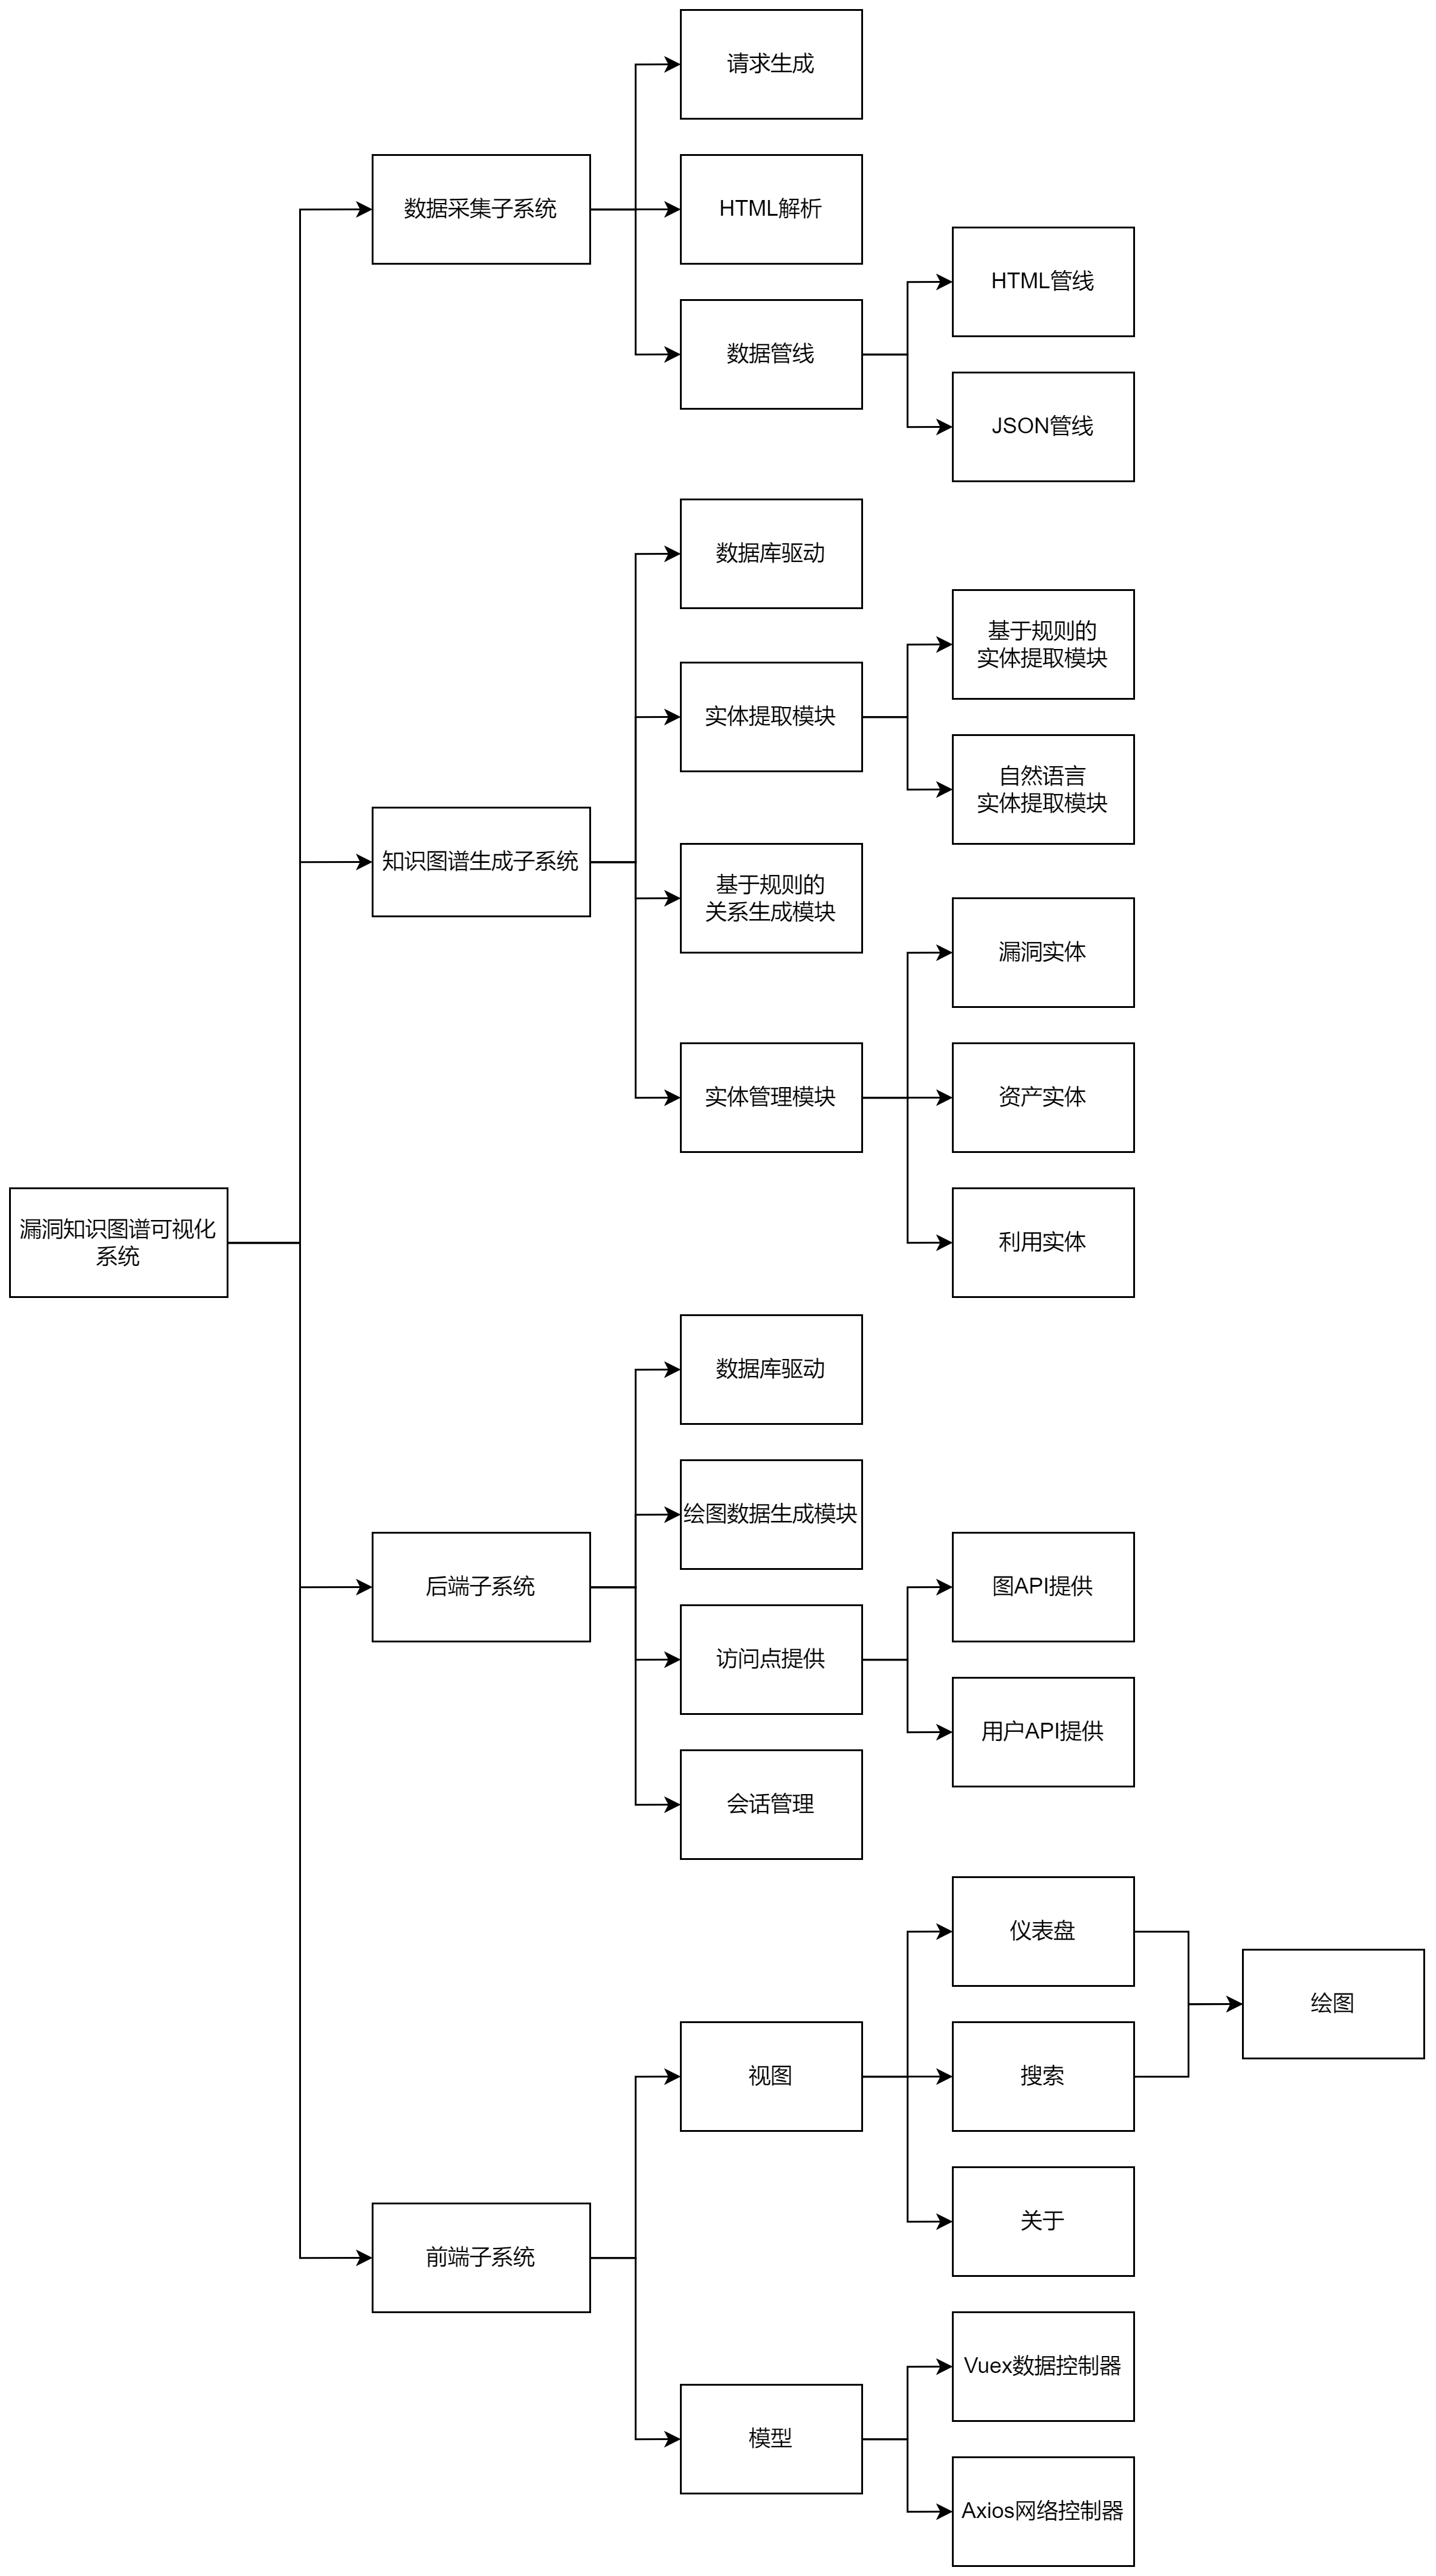
\includegraphics[height=0.97\textheight]{pictures/CyKG_OrgChart-中文.png}
	\caption{系统功能模块设计图}
	\label{CyKG_OrgChart}
\end{figure}

\subsection{数据采集子系统}

主要实现 Web 爬虫服务,包括请求生成器、异构数据解析器、异构数据管线三个模块。其中异构数据解析器包含包含 HTML 解析器、JSON 解析器、csv 解析器、gzip 解析器等。异构数据管线包含与异构数据解析器对应的各类数据管线。

请求生成器根据 csv 索引生成爬虫请求链接,交由 Scrapy Spider 进行并发爬虫。

异构数据解析器负责使用对应解析器解析 Spider 爬虫返回的网络数据,传递给异构数据管线。此外,异构数据解析器中的 HTML 解析器应用在一些网站的爬虫任务时,还会解析页面上包含``下一页''等元素的 <a> 标签,通过 yield 将其中 href URL 交给请求生成器,生成新的爬虫请求。

异构数据管线负责接收其对应的数据解析器传来的数据,提取其中需要的信息进行格式转换等处理,填充固定格式的 Python Dictionary,再调用持久化子系统中的数据库控制器对象,将请求原始数据与 Dictionary 分别存储至不同的 MongoDB 数据库集合(Collection)中持久化存储,形成原始数据,完成数据采集工作。

\subsection{知识图谱构建子系统\label{知识图谱构建子系统}}

主要实现知识图谱构建服务,包含实体生成模块、基于规则的关系生成模块、关系融合模块。

\subsubsection{本体定义\label{本体定义}}

采用自顶向下方法构建信息安全漏洞领域知识图谱,首先需定义信息安全漏洞本体。调研归纳与信息安全漏洞相关概念及术语如下:
\begin{itemize}
	\item Vulnerability:漏洞或脆弱性,指计算机信息系统在需求、设计、实现、配置等方面的缺陷,漏洞被利用会导致计算机信息系统在数据的保密性、完整性、可用性、访问控制等方面面临威胁。\cite{cnnvd_vul_category}
	\item Asset:资产,信息技术系统、软甲和软件包等产品统称为资产。CPE 项目列举官方资产列表。
	\item Exploit:对漏洞的利用代码,通常是程序片段,提供对漏洞利用的概念验证。
	\item CVE:公共漏洞和暴露,提供一个命名字典,为广泛认同的信息安全漏洞或已经暴露的弱点给出一个公共名称,收集各种信息安全弱点及漏洞并给予编号以便于公众查阅。\cite{cve_intro}
	\item CPE:通用平台枚举,是信息技术系统、软件和软件包的结构化命名方案。基于统一资源标识符(URI)的通用语法,CPE 提供一个官方 CPE 产品字典,枚举商定的官方 CPE 名称列表。\cite{cpe_intro}
	\item CWE:通用弱点枚举,是一个社区开发的具有安全影响的常见软硬件弱点类型列表。标准化分类列举描述软硬件实现、代码、设计或架构中的缺陷、故障、漏洞或其他错误。\cite{cwe_intro}
	\item CVSS:通用漏洞评分系统,提供一种评分方法来捕捉漏洞的主要特征并反映其严重性。评分可以转换为定性的表示(高、中、低等)。\cite{cvss_intro}
\end{itemize}

根据以上概念可推导关系:Vulnerability 漏洞具备 CVE 作为唯一标识、具备 CVSS 属性评价漏洞严重性、漏洞产生的原因对应一个或多个 CWE;Asset 资产具备 CPE 作为唯一标识,资产具有漏洞、漏洞影响资产;Exploit 利用代码无通用唯一标识、一个利用代码有时可对应多个漏洞,利用代码利用漏洞、攻击资产。

图\ref{pictures/CyKG_Entity-Ontology.png}所示为信息安全漏洞本体,给出了实体定义及关系定义。分为  漏洞 Vulnerability、资产 Asset、利用 Exploit 三类实体,图中给出每类实体作为索引的属性域,该属性具有唯一性。三类实体之间利用上述联系,定义关系边连接。详见下述章节 \ref{实体生成} \nameref{实体生成}与 \ref{关系生成} \nameref{关系生成}。

\buptfigure[width=0.8\textwidth]{pictures/CyKG_Entity-Ontology.png}{信息安全漏洞本体定义}{pictures/CyKG_Entity-Ontology.png}

\subsubsection{实体生成\label{实体生成}}

目前包含基于规则的实体生成子模块,未来可引入基于深度学习模型的自然语言实体生成子模块。基于规则的实体生成模块应用自顶向下人工构建的互联网信息安全漏洞本体规则,从结构化数据抽取实体及其属性。前述数据采集子系统获得的结构化数据,经处理后包含根据规则定义的属性域,如下:
\begin{itemize}
	\item 漏洞:\lstinline|cve_id|,格式为 \lstinline|CVE-[0-9]+-[0-9]+|
	\item 资产:\lstinline|cpe23uri|,格式如代码 \ref{lst:cpe23regex} 所示。
	\item 利用代码:\lstinline|edb_id|,为 exploit-db.com 的数字序号。因利用代码无通用标识符,需使用 \lstinline|UUIDv4| 方法生成本系统内使用的标识符。
\end{itemize}

\begin{lstlisting}[caption={CPE 2.3 格式正则表达式},label={lst:cpe23regex},breaklines,style=lgeneral]
	cpe:2\.3:[aho\*\-](:(((\?*|\*?)([a-zA-Z0-9\-\._]|(\\[\\\*\?!"#$$%&'\(\)\+,/:;<=>@\[\]\^`\{\|}~]))+(\?*|\*?))|[\*\-])){5}(:(([a-zA-Z]{2,3}(-([a-zA-Z]{2}|[0-9]{3}))?)|[\*\-]))(:(((\?*|\*?)([a-zA-Z0-9\-\._]|(\\[\\\*\?!"#$$%&'\(\)\+,/:;<=>@\[\]\^`\{\|}~]))+(\?*|\*?))|[\*\-])){4}
\end{lstlisting}

生成方法根据属性域,区分实体类型,调用相应方法从文档提取属性,调用持久化子系统的数据库控制对象将结点存入 Neo4j 数据库。来自不同数据源的实体存储在 MongoDB 不同集合中,如来自 NVD JSON API 的数据存储于 \lstinline|nvd_json| 集合中。针对每个数据库集合,在 Python 中实现一个实体生成方法。如 \lstinline|nvd_json| 集合对应方法为遍历数据库存储的文档,对于每个文档,提取其 \lstinline|cve_id, cwe_id, desc, impact{}, references[], publish_date, last_update_date, version, timestamp| 作为 Vulnerability 实体的属性,提取其 \lstinline|cpe23uri| 作为 Asset 实体的属性。对于仅包含资产信息的 \lstinline|cpe| 集合,将每个文档生成一个 Asset 实体,并与已经存在的 \lstinline|cpe23uri| 相同的实体融合。

\subsubsection{关系生成\label{关系生成}}

基于规则的关系生成模块根据信息安全漏洞本体所表示关系,在 Neo4j 数据库中匹配对应结点,在两个结点间生成对应的边,并为其添加属性:
\begin{itemize}
	\item 资产$-[$具有$]->$漏洞,漏洞$-[$影响$]->$资产
	\item 利用代码$-[$攻击$]->$资产,资产$-[$被攻击$]->$利用代码
	\item 漏洞$-[$被利用$]->$漏洞代码,利用代码$-[$利用$]->$漏洞
\end{itemize}

因知识图谱中预计将有一百万个结点,使用最细粒度将每个漏洞结点与每个资产结点连接将产生超过一亿条边,这对于本项目的性能要求而言是不现实的。因此,关系生成模块会使用前述步骤生成的资产家族结点,在漏洞结点与漏洞结点所包含的受影响资产列表中的每条正则匹配项所匹配到的资产对应的资产家族之间添加关系。为了维持该关系指向资产的语义准确,将正则匹配到的资产列表作为属性添加到该关系边之上:
\begin{itemize}
	\item 资产家族$-[$具有$]->$漏洞,漏洞$-[$影响$]->$资产家族
	\item 资产$-[$是子级$]->$资产家族,资产家族$-[$是父级$]->$资产
	\item 利用代码$-[$攻击$]->$资产家族,资产家族$-[$被攻击$]->$利用代码
	\item 漏洞$-[$被利用$]->$漏洞代码,利用代码$-[$利用$]->$漏洞
\end{itemize}

如此可将构建图谱所需关系数量从亿级降低到百万级,在不损失语义的情况下有效提高查询效率,减小数据库体积。

\subsubsection{关系融合}

关系融合模块作为适配使用深度学习模型进行命名实体识别结点生成与关系抽取方案的模块,当前仅在系统数据加工管线中留有接口,以备未来扩展需要。当前系统的结构化数据实体与关系生成已经实现实体结点和关系的消除二义性,因此无需实现关系融合模块。

\subsection{后端服务子系统}

主要负责提供后端 Web API、对知识图谱的数据进行转换处理、调度各服务运行。包括绘图数据生成模块、Web API 访问点、APScheduler 调度模块。

Web API 访问点由 Flask 支持,使用 Flask 的 Blueprint 功能对注册在 RESTful API 根路径下的第一级 API 进行分组管理,实现模块化设计。在某个 Route 收到请求时,根据用户请求内容,将请求参数作为 CQL 参数,调用持久化层数据库控制对象对数据库进行操作,增删查改知识图谱中的结点和关系。若是可视化相关的 Route,则会对查询到的数据调用绘图数据生成模块进行转换。

绘图数据生成模块将存储在 Neo4j 数据库中的知识图谱数据转化为 ECharts 绘图库可以使用的数据格式。

APScheduler 调度模块:通过调用数据采集子系统和知识图谱构建子系统提供的 Runner 方法,实现爬虫、更新图谱的定时运行。

\subsection{前端子系统}

前端子系统负责管理用户运行时相关数据、通过 UI 向用户展示信息。使用 Vue.js 的 MVVM 架构,主要包含视图与模型两个组成部分。

% 视图包含概览、可视化、搜索、控制台、关于五部分。
视图包含概览、可视化、搜索、关于四部分。

\begin{itemize}
	\item 概览视图为用户提供知识图谱信息概览,包含列表形式的数据展现,以及统计图表形式的数据可视化。
	\item 可视化视图是一个全屏视图,通过该视图用户可以一览知识图谱全貌。
	\item 搜索视图支持用户在图谱中搜索感兴趣的内容,并将搜索结果以力引导图可视化的形式展示。
	      % \item 控制台视图向用户展示当前系统运行状态,如数据更新日期、当前系统正在运行的任务、任务进度等。管理员用户可以手动控制各个任务的开始或停止。
	\item 关于视图展示本系统介绍信息及用户指南。
\end{itemize}

模型主要包含 Vuex 数据控制器、Axios 网络控制器两部分。Vuex 数据控制器统一管理前端子系统的数据与状态,是前端子系统的``Single Source of Truth'',为视图的响应式显示提供数据源,还包含在前端对数据进行简单处理功能。Axios 网络控制器封装一个 httpCliet 对象,以及若干与后端通信的方法。Vuex 数据控制器可以调用 Axios 网络控制器,从后端获取数据,更新 Vuex Store 中的状态。

\subsection{数据库设计}

\subsubsection{MongoDB}

图\ref{CyKG_Entity-Mongo}所示为 MongoDB 数据模式图。由于 MongoDB 支持动态 DDL,因此数据库在本项目开发后期共有 7 个集合。
\begin{itemize}
	\item cpe:存储从 XML 解析的 cpe 资产数据。
	\item edb{\_}html:存储从 exploit-db.com 爬虫获得的 HTML 原始数据。
	\item edb{\_}json:存储从 exploit-db.com HTML 数据处理得到的 JSON 数据。
	\item cve{\_}html:存储从 cvedetails.com 爬虫获得的 HTML 原始数据。
	\item cve{\_}json:存储从 cvedetails.com HTML 数据处理得到的 JSON 数据。
	\item nvd{\_}json{\_}src:存储从 nvd.nist.gov 数据接口获得的 JSON 原始数据。
	\item nvd{\_}json:存储从 nvd.nist.gov JSON 数据处理得到的 JSON 数据。
\end{itemize}

\buptfigure[height=0.95\textheight]{pictures/CyKG_Entity-Mongo.png}{MongoDB 数据模式图}{CyKG_Entity-Mongo}

\subsubsection{Neo4j}

图\ref{CyKG_Entity-Neo}所示为 Neo4j 数据模式图,同时也是知识图谱实体与关系模式图。

\buptfigure[width=\textwidth]{pictures/CyKG_Entity-Neo.png}{Neo4j 数据模式图}{CyKG_Entity-Neo}

\nameref{CyKG_Entity-Neo}中,\lstinline|Vulnerability, Asset Family, Asset, Exploit| 为主要实体结点。\lstinline|Vulnerability, Asset, Exploit| 为章节 \ref{本体定义} \nameref{本体定义}所述信息安全漏洞本体的实体;\lstinline|Asset Family| 结点是属于同一类型、同一制造商、同一产品的资产的集合,是一个抽象的概念实体。

\lstinline|Vulnerability| 漏洞实体的 \lstinline|cve_id| 属性为索引,\lstinline|version| 标识数据格式版本,\lstinline|timestamp| 记录数据更新时间,\lstinline|vuln, assets[]| 为复合属性。\lstinline|vuln| 复合属性记录漏洞相关信息,\lstinline|cve_id| 与索引属性相同,\lstinline|cwe_id| 为漏洞的 CWE 类型,\lstinline|desc| 为漏洞的自然语言描述,\lstinline|impact{}| 为元组复合属性,记录漏洞的 CVSS 信息,\lstinline|references| 为列表复合属性,记录漏洞相关参考资料。\lstinline|assets[]| 为列表复合属性,包含一系列用于匹配资产的正则表达式。

\lstinline|Asset| 为资产实体,索引属性 \lstinline|cpe23uri| 为资产的 CPE 标识 URI;\lstinline|field{}| 元组复合属性对应 \lstinline|cpe23uri| 的各部分语义;\lstinline|references[]| 列表复合属性记录一系列关于此资产的参考资料链接及资料类型标签;\lstinline|title| 为资产的自然语言名称,\lstinline|timestamp| 记录数据更新时间。

\lstinline|Asset Family| 为资产家族实体,为了解决漏洞影响资产过多而导致关系数量庞大的问题而提出。资产家族的索引属性 \lstinline|cpe23uri| 同为 CPE 标识 URI,与资产 \lstinline|Asset| 的 \lstinline|cpe23uri| 属性区别在于,资产家族的该属性仅有 \lstinline|part, vendor, product| 三个字段。

\lstinline|Exploit| 为利用代码实体,\lstinline|edb_id| 为 exploit-db.com 的数字序号;\lstinline|title| 为利用代码描述性自然语言标题;\lstinline|author| 为代码作者;\lstinline|type| 为代码执行类型,分类如网络、邻接、本地、物理等;\lstinline|platform| 为利用代码或漏洞的运行平台;\lstinline|date| 为该段代码的更新日期;\lstinline|code| 为代码文本;\lstinline|cve_ids[]| 是列表复合属性,为 \lstinline|cve_id| 组成的列表,记录与此利用相关的漏洞编号。

全部实体均有 \lstinline|eid| 索引属性,\lstinline|eid| 即 entity id,使用 \lstinline|UUIDv4| 方法生成,保证唯一性。

实体之间的关系为:

\begin{lstlisting}[label={lst:neo4j_rels},breaklines,style=lgeneral]
	Vulnerability-[Affects]->AssetFamily, AssetFamily-[Has]->Vulnerability
	Exploit-[Exploits]->Vulnerability, Vulnerability-[ExploitedBy]->Exploit
	AssetFamily-[AttackedBy]->Exploit, Exploit-[Attacks]->AssetFamily
	Asset-[ChildOf]->AssetFamily, AssetFamily-[ParentOf]->Asset
\end{lstlisting}

所有关系都具有 \lstinline|rid| 索引属性即 relationship id 作为唯一标识。\lstinline|Has/Affects| 关系具有的属性为 \lstinline|assets[]| 列表复合属性记录该条边代表的受影响资产正则匹配表达式,\lstinline|asset_cnt| 属性
记录满足正则匹配规则的全部资产数量。\lstinline|Attacks/AttackedBy| 关系的属性与 \lstinline|Has/Affects| 相同。

\subsection{系统接口设计}

% 表\ref{api_table}展示了系统接口设计。
% \begin{bupttable}{系统接口设计}{api_table}
% 	\begin{tabularx}{\textwidth}{llX}
% 		\toprule
% 		\textbf{类别} & \textbf{路径}             & \textbf{描述}                                         & \textbf{返回值} \\ \midrule
% 		              & /<path>                   & 前端路由路径                                          & 1               \\ \cmidrule(l){2-3}
% 		              & GET /api/graph/           & 获取知识图谱统计信息                                  & 2               \\ \cmidrule(l){2-3}
% 		前端          & GET /api/graph/<limit>    & 获取与<limit>个漏洞结点相关联的结点或关系组成的子图谱 & 3               \\ \cmidrule(l){2-3}
% 		              & GET /api/search/<keyword> & 搜索与<keyword>关键字相关的结点或关系                 & 4               \\ \bottomrule %\midrule
% 	\end{tabularx}
% \end{bupttable}
类别:前端路由
\begin{itemize}
	\item \lstinline|/welcome|:欢迎页面
	\item \lstinline|/overview|:概览页面
	\item \lstinline|/vis|:可视化页面
	\item \lstinline|/search|:搜索页面
	\item \lstinline|/about|:关于页面
\end{itemize}

类别:后端接口
\begin{itemize}
	\item \lstinline|/api/graph/|
	      \begin{itemize}
		      \item 方法:GET
		      \item 参数:无
		      \item 描述:获取知识图谱统计信息,包含漏洞数量、各类别资产数量、利用数量等
		      \item 返回值:含 \lstinline|vul, asset, exploit| 三个键的 JSON,每个键对应的值为实体相关数据 JSON
	      \end{itemize}
	\item \lstinline|/api/graph/<limit>|
	      \begin{itemize}
		      \item 方法:GET
		      \item 参数:\lstinline|limit|,整数字符串
		      \item 描述:获取与<limit>个漏洞结点相关联的结点或关系组成的子图谱
		      \item 返回值:含 \lstinline|categories, nodes, links| 三个键的 JSON,每个键对应的值为一个列表,列表中的每个元素代表一个类别、一个结点或一个关系
	      \end{itemize}
	\item \lstinline|/api/search/<keyword>|
	      \begin{itemize}
		      \item 方法:GET
		      \item 参数:\lstinline|keyword|,搜索关键字,字符串
		      \item 描述:搜索关键字相关的漏洞、资产、利用结点或关系
		      \item 返回值:同 \lstinline|GET /api/graph/<limit>|
	      \end{itemize}
\end{itemize}

\section{系统详细设计}

\subsection{开发环境配置}

\begin{itemize}
	\item 操作系统:Ubuntu 20.04,Windows 11 Pro
	\item 数据采集子系统:Python 3.8,Scrapy 2.6
	\item 知识图谱构建子系统:Python 3.8,Ray 1.11.1,uuid 1.3
	\item 持久化子系统:Python 3.8,Py2neo 2021.2.3,Pymongo 3.12,Neo4j 4.4
	\item 后端服务子系统:Python 3.8,Flask 2.0,flask-cors 3.0
	\item 前端子系统:JavaScript ES6,Vue 2.6,Vuetify 2.6,ECharts 5.3.2,vue-axios 3.4,Vuex 3.4,Moment 2.29.3,Lodash 4.17.21
\end{itemize}

\subsection{各核心功能模块详细设计}

\subsubsection{类图}

\buptfigure[width=\textwidth]{pictures/CyKG_Class-DataCollection.png}{数据采集子系统类图}{CyKG_Class-DataCollection}

图\ref{CyKG_Class-DataCollection}所示为数据采集子系统类图。其中 \lstinline|Item| 的数据模式与 MongoDB 里同名集合模式相同。

\lstinline|Spider| 类继承自 \lstinline|scrapy.spider| 类,包含异构数据源站点爬虫实现,内置请求生成器及异构数据解析器。

\lstinline|Item| 类为 Scrapy 内置数据对象,可用于定义数据模型并且在 \lstinline|Spider| 与 \lstinline|Pipeline| 间传递信息。

\lstinline|Pipeline| 类为异构数据管线。\lstinline|GzFilePipeline| 继承自 \lstinline|scrapy.FilePipeline| 数据管线,其他管线为单独实现。

% \begin{figure}[H]
% 	\centering
% 	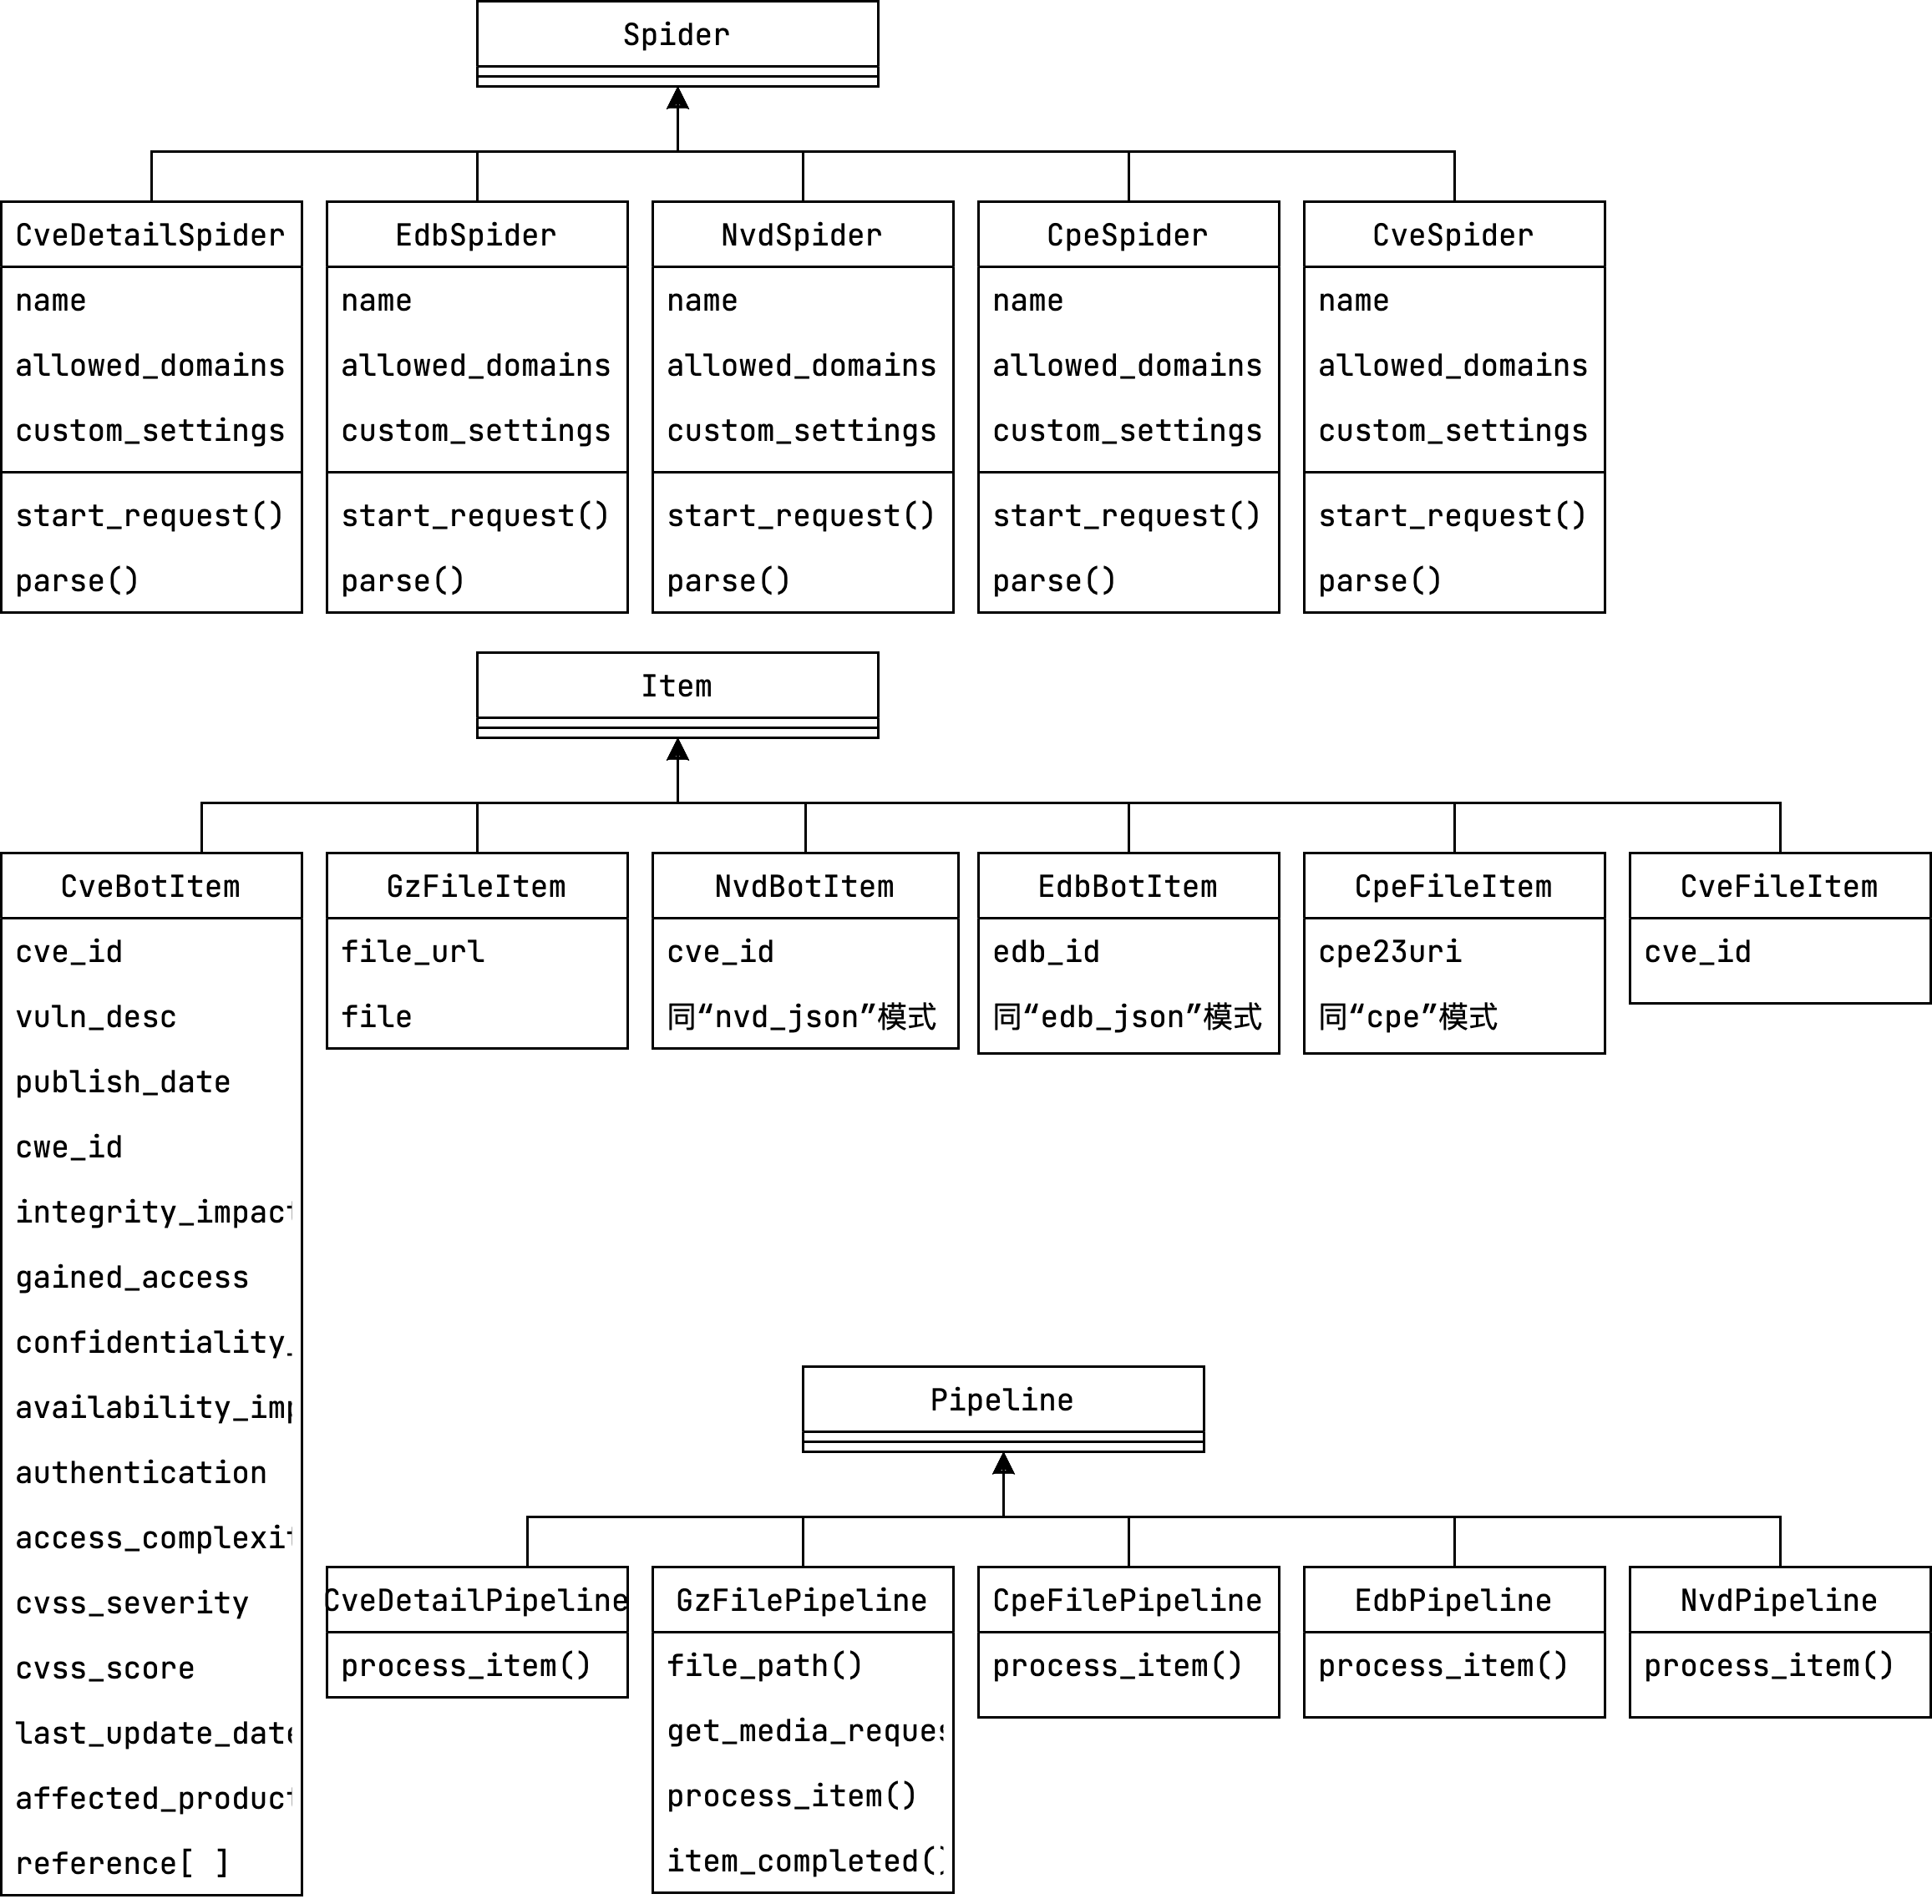
\includegraphics{pictures/CyKG_Class-DataCollection.png}
% 	\caption{Write some caption here}
% \end{figure}

\buptfigure[width=\textwidth]{pictures/CyKG_Class-KnowledgeGraphGeneration.png}{知识图谱构建子系统类图}{CyKG_Class-KnowledgeGraphGeneration}

图\ref{CyKG_Class-KnowledgeGraphGeneration}所示为知识图谱构建子系统类图。

\lstinline|init_kg()| 为模块的函数入口,可被调度系统调用进行图谱更新。其中 \lstinline|init_nodes(), init_rels()| 为支持 Ray 框架的并行化函数,它们内部各自又实现了生成漏洞结点、生成资产结点、生成漏洞到资产家族关系等一系列并行化函数,用于并发构建知识图谱。

\lstinline|VulnEntity| 则实现了一个互联网安全漏洞本体类。

\buptfigure[height=0.7\textheight]{pictures/CyKG_Class-Database.png}{持久化子系统类图}{pictures/CyKG_Class-Database.png}

图\ref{pictures/CyKG_Class-Database.png}所示为持久化子系统类图。

持久化子系统主要包含 \lstinline|MyMongo, MyNeo| 两个数据库控制器类。在 \lstinline|__init__()| 方法中实现了单例模式;使用自带连接池,实现若干用于读写数据库的方法。

\buptfigure[width=\textwidth]{pictures/CyKG_Class-Backend.png}{后端服务子系统类图}{CyKG_Class-Backend}

图\ref{CyKG_Class-Backend}所示为后端服务子系统类图。

\lstinline|Flask| 对象中注册了 \lstinline|CORS| 中间件,包含 \lstinline|User, Graph| 两个模块化的蓝图。\lstinline|User| 蓝图注册用户相关 API,\lstinline|Graph| 蓝图注册知识图谱相关 API。后端服务启动,Flask 类实例化时调用 \lstinline|APScheduler| 模块的初始化方法,向 Flask 实例挂载计划任务和响应的调度器。

\lstinline|DataConverter| 是绘图数据生成器模块,包含将结点、关系和若干预定义三元组从知识图谱数据结构转换为 ECharts 可用数据结构的方法。

\lstinline|APScheduler| 是后端子系统的调度模块,使后端子系统能控制数据采集子系统、知识图谱构建子系统的运行或停止。

\subsubsection{功能时序图}

图\ref{CyKG_Sequence-UserSequence}所示为通用状态下用户操作前端发起请求的时序图。

\buptfigure[width=0.9\textwidth]{pictures/CyKG_Sequence-UserSequence.png}{用户请求功能时序图}{CyKG_Sequence-UserSequence}

用户上线后,前端页面被挂载时调用钩子函数向后端发送初始请求。初始请求包含用户信息、系统的状态、数据更新的时间等。这些信息将会在页面顶部一条高 24px 的信息栏上常驻显示。同时,向 Vuex 注册定时器及回调函数,周期性发送心跳包更新数据。

用户进行操作(点击按钮、切换视图页面、搜索图谱等)时,会发送两个请求。一是立即触发定时器回调函数,发送系统状态更新请求。二是发送操作相关请求。系统状态更新请求回调后会更新 Vuex 中的数据,前端视图层响应式更新显示。操作相关请求回调后,更新 Vuex 中的数据,根据操作类型调用 ECharts 实例的重绘方法,重绘视图层 canvas。

由于本系统多数流程为全自动控制,且与用户操作完全异步,不作功能时序图展示。数据采集子系统与知识图谱构建子系统的工作流程可见图 \ref{pictures/Impl_DataCollection.png} \nameref{pictures/Impl_DataCollection.png}与图 \ref{pictures/Impl_KGCreation.png} \nameref{pictures/Impl_KGCreation.png}。

\chapter{系统实现}

\section{工具模块}

\subsection{根目录模块实现 bot{\_}root{\_}dir.py}

本模块位于项目根目录下。\lstinline[style = python]|get_bot_root_dir()| 方法使用 pathlib 的 \lstinline[style = python]|Path(__file__).parent| 方法获得项目根目录的路径,使得本项目内代码全部使用平台无关的相对路径,从而能在 Linux、macOS、Windows 等多种系统平台运行,保证可移植性。

本模块内包含许多路径相关的方法,如 \lstinline|get_source_data_dir(), get_cve_data_dir(), get_log_dir()| 等。这些方法接受字符串形式的路径参数,返回 \lstinline|Path| 对象。通过传入参数,控制系统生成的文件存放的位置,若目录不存在,则会自动创建所需目录。

本系统所有涉及文件系统的模块都依赖于此模块。

\subsection{日志模块实现 logger{\_}factory.py}

在 Python Logging 模块基础上重新实现了自定义的日志功能。具有 \lstinline|init_log_dir(), setup_logger(), mylogger(), loggers={}| 等方法和属性。

\lstinline|init_log_dir()| 接受字符串路径可选参数,初始化日志记录路径。若参数为空,则使用默认路径。

\lstinline|setup_logger(name, log_folder=None, lvl_file=None, lvl_stdout=None)| 是一个工厂函数,创建一个新的 Logger 对象,根据参数设置 \lstinline|FileHandler(), StreamHandler()|。支持自定义日志路径、文件名称和不同 Handler 使用不同记录等级。

\lstinline[style = python]|mylogger()| 实现 logger 对象的单例模式\cite{singleton_design_pattern}。利用 Python 模块引入为单例的特性,使得在同一模块内多次调用相同 \lstinline[style = python]|<name>| 的 \lstinline[style = python]|mylogger()| 会返回相同的 Logger 对象。当第一次调用 \lstinline|mylogger(<name>)| 时,会调用 \lstinline|setup_logger()| 创建一个新的 Logger 对象,并且将其保存在全局变量 loggers 字典内。之后调用同样的 \lstinline|mylogger(<name>)| 时,会根据 \lstinline|<name>| 从 loggers 字典查找对应的 Logger 对象并返回。

在一个模块内首次调用 \lstinline[style = python]|mylogger(<name>)| 会初始化日志,添加日志的文件控制器与标准输出控制器,并且设定输出日志文件位置,以``本模块名 + 当前时分秒''命名。后续再次调用 \lstinline[style = python]|mylogger(<name>).log()| 会使用首次创建的 logger 对象进行日志记录。

\subsection{环境配置文件 secret.py}

以 Python 变量的形式存储 MongoDB 与 Neo4j 数据库的用户名、密码、数据库名、连接 URL 等信息,和一些私有 API 的密钥等信息。此文件被 \lstinline|.gitignore|,不会同步到远程仓库。

\section{数据采集子系统}

数据采集子系统工作流程如 \ref{pictures/Impl_DataCollection.png} 所示。

\buptfigure[width=\textwidth]{pictures/Impl_DataCollection.png}{数据采集子系统工作流程图}{pictures/Impl_DataCollection.png}

\subsection{Spider 模块实现}

每个 Spider 继承自\lstinline[style = python]|scrapy.Spider| 类,重写了父类的 \lstinline[style = python]|__init__(), start_requests(),  parse()| 方法。

\subsubsection{初始化 {\_\_}init{\_\_}() 实现}
% \subsubsection{\textunderscore \textunderscore init\textunderscore \textunderscore}

\lstinline[style = python]|__init__()| 方法完成 Spider 类的初始化工作。在调用父类的 \lstinline|super.__init__()| 方法之后,调用本系统基于 Python Logging 模块重新自定义封装的 \lstinline[style = python]|mylogger(<name>)| 函数初始化 logger。

\subsubsection{发起请求 start{\_}requests() 实现}
% \begin{lstlisting}[style = python]
% 	for x in range(101):
% 		print('fizz'[x%3*4:] + 'buzz'[x%5*4:] or x)
% 		print('Hello world!') yield scrapy.Request(url=url, callback=self.parse) yield scrapy.Request(url=url, callback=self.parse)
% \end{lstlisting}
\lstinline[style = python]|start_requests()| 方法描述发起请求的步骤。

对于需要 cve id 索引的 Spider 如 \lstinline[style = python]|CveDetailSpider(scrapy.Spider)|,使用 Pandas 库的 \lstinline[style = python]|read_csv()| 方法,设置 \verb|chunksize| 数值和 \verb|iterator=True|,分块迭代读取 csv 文件。对每一行 cve id,生成所需 URL 并使用 \lstinline[style = python]|yield scrapy.Request(url=url, callback=self.parse)| 发出请求。

对于需要从爬取页面中获得下一页 URL 的 Spider 如 \lstinline[style = python]|EdbSpider(scrapy.Spider)|,\linebreak \lstinline[style = python]|start_request()| 方法中仅指定初始页面发出请求,在解析收到的 response 时处理下一页面的链接,并发出请求。

对于采用 JavaScript 动态加载页面的站点如 exploit-db.com,使用将 playwright 无头浏览器与 Scrapy 框架集成的 scrapy-playwright 库,对爬取到的 HTML 页面及其 JavaScript 代码进行渲染,将渲染生成的 DOM 返回给 Spider 的 \lstinline[style = python]|parse()| 方法。

\subsubsection{解析数据 parse() 实现}

\lstinline[style = python]|parse()| 方法实现对请求返回数据的解析。

对于返回数据为 HTML 文档类型,使用 BeautifulSoup 库加载 DOM 进行解析。使用 \lstinline[style = python]|soup.select_one()| 方法配合 CSS 选择器提取所需标签的内容。对于需要在页面上查找下一请求 URL 的站点,使用 \lstinline[style = python]|yield scrapy.Request()| 方法发出请求。将解析出的数据封装在 \lstinline[style = python]|scrapy.Item| 类中,使用 \lstinline[style = python]|yield item| 方法将数据传递给对应数据管线。

对于返回数据为 JSON 类型,使用 \lstinline[style = python]|response.json()| 获取返回数据,将其作为参数实例化 Item 对象,传递给 JSON 数据管线。

对于单个请求返回数据为 Gz 压缩的 XML 类型,使用工具模块 \lstinline[style = python]|gz.py| 的 \lstinline[style = python]|un_gz()| 方法解压文件得到 XML,并使用 lxml 模块的 \lstinline[style = python]|etree.iterparse(filepath, tag='')| 方法迭代遍历该 XML 文件,填充 item,最终调用持久化子系统的数据库控制对象提供的 \lstinline[style = python]|save_cpe()| 方法存储。

将以上代码段包裹在 Python 的 \lstinline|try...except...finally...| 语句内,使日志模块能正常 \lstinline|catch| 抛出的错误,并使程序不中断继续运行。

\subsection{Item Pipeline 模块实现}

每个 Pipeline 类实现一个 \lstinline[style = python]|process_item()| 方法,同时在 Spider 的 \lstinline[style = python]|custom_settings| 内设置对应的 Pipeline 类。Scrapy Engine 将 Spider 内 \lstinline[style = python]|yield item| 发送给 Pipeline 对象进行处理。

GzPipeline 负责处理压缩成 Gzip 格式的 cve 与 cpe XML 文件。将其解压并返回解压后文件的路径。

NvdPipeline 负责处理 NVD API 提供的 JSON,提取数据并调用持久化子系统的数据库控制对象提供的 \lstinline|save_nvd_src()| 方法存储原始数据,使用 \lstinline|save_nvd()| 方法存储处理过的数据。

其余 Pipeline 功能类似,根据爬取站点不同,实现有所不同。

\subsection{其他模块实现}

\begin{itemize}
	\item \lstinline|scrapy.cfg|:存放 Scrapy 项目设置选项,如默认设置文件、项目名称等。
	\item \lstinline|settings.py|:Python 变量形式存放 Scrapy 爬虫设置选项,如并发度、请求延时、User-Agent 等。
	\item \lstinline|crawl_runner| 目录:包含 \lstinline|crawl_cpe.py, crawl_nvd.py, crawl_edb.py| 等。使用\linebreak \lstinline|scrapy.cmdline.execute()| 方法运行爬虫程序。可以被调度模块调用,实现全自动爬虫。
\end{itemize}

\section{知识图谱构建子系统}

数据采集子系统工作流程如 \ref{pictures/Impl_KGCreation.png} 所示。

\buptfigure[width=\textwidth]{pictures/Impl_KGCreation.png}{知识图谱构建子系统工作流程图}{pictures/Impl_KGCreation.png}

\subsection{实体生成}

% 实体生成模块主要包含 \lstinline|init_nodes(vul_num=0, asset_num=0, exploit_num=0)|,\lstinline|init_vul_ray(skip, _limit)|,\lstinline|init_asset_ray(skip, _limit)|,\lstinline|init_exploit_ray(skip, _limit)|,\lstinline|init_asset_family_ray(skip, _limit)|,\lstinline|get_step(num)| 几个方法。
实体生成模块主要包含
\begin{lstlisting}[style=lgeneral]
	init_nodes(vul_num = 0, asset_num = 0, exploit_num = 0)
	init_vul_ray(skip, _limit)
	init_asset_ray(skip, _limit)
	init_exploit_ray(skip, _limit)
	init_asset_family_ray(skip, _limit)
	get_step(num)
\end{lstlisting}
几个方法。

\subsubsection{init{\_}nodes() 实现}

\lstinline|init_nodes(vul_num, asset_num, exploit_num)| 方法接受可选参数漏洞数量、资产数量、利用代码数量,若参数不为零,则将数据根据并行度参数分割并行处理,使用 \lstinline|ray.get()| 方法等待并行处理结束。示例代码如下:
\begin{lstlisting}[style=lgeneral]
	'''Ensure Vulnerability, Asset, Exploit nodes exist'''
	arr = [init_vuln_ray.remote(skip=i, _limit=get_step(vuln_num) + 1) for i in range(0, vuln_num, get_step(vuln_num))]
	arr.extend([init_asset_ray.remote(skip=i, _limit=get_step(asset_num) + 1) for i in range(0, asset_num, get_step(asset_num))])
	arr.extend([init_exploit_ray.remote(skip=i, _limit=get_step(exploit_num) + 1) for i in range(0, exploit_num, get_step(exploit_num))])
	ray.get(arr)
	'''Ensure Asset:Family nodes exist'''
	family_id = [init_asset_family_ray.remote(skip=i, _limit=get_step(asset_num) + 1) for i in range(0, asset_num, get_step(asset_num))]
	ray.get(family_id)
\end{lstlisting}

若不传入漏洞数量等参数,默认使用单线程串行处理。

\subsubsection{漏洞实体生成的实现 init{\_}vul{\_}ray()\label{subsubsec:vul}}

\lstinline|init_vul_ray(skip, _limit)| 方法用于生成漏洞实体结点。\lstinline|skip| 参数指定跳过数据库查询结果中的前多少个记录,\lstinline|_limit| 参数指定最多处理多少个数据库查询结果。两个参数配合使用,可以实现从第 \lstinline|<skip>| 个记录开始,处理 \lstinline|_limit| 个记录。从而实现并行化处理。伪代码:
\begin{lstlisting}[style=lgeneral]
	cursor = mongo.get_nvd().skip(skip).limit(_limit) # 获取 MongoDB 数据库查询指针
	for doc in cursor:
		try:
			doc = split_properties(doc, api_ver=doc['api_ver']) # 根据 API 版本,提取属性
			neo.add_vul(doc) # 调用数据库控制对象添加 doc
		except BaseException as e:
			# 异常处理
	mongo.close_db() # 释放数据库连接
\end{lstlisting}

创建一个持久化子系统数据库控制器单例对象 \lstinline|_mg = MyMongo()|,调用方法 \lstinline|get_nvd(cve_id = None)| 不传入参数,获取 MongoDB 数据库中全部 NVD 数据的迭代指针对象。根据传入参数从指定位置迭代处理查询记录。

对于每个记录,调用 \lstinline|split_properties(doc, api_ver = ApiVersion.NVDv1)| 方法,\lstinline|ApiVersion| 是一个自定义枚举类型,用于枚举不同的数据 API 类型。这个方法根据不同的 \lstinline|api_ver| 使用不同的处理方式,将原始数据中的信息分割为不同语义,并将可用于索引的属性域提至外层。随后调用循环体外创建的持久化子系统数据库控制器单例对象 \lstinline|neo = MyNeo()| 将实体结点不重复地加入知识图谱中。

将以上循环体内代码包裹在 \lstinline|try...except...finally...| 语句内保证正确处理异常并且程序不会意外中断。此外,在处理开始、循环体中间、处理结束均使用前述日志模块的 \lstinline|mylogger()| 方法进行日志输出。

\subsubsection{资产实体生成的实现 init{\_}asset{\_}ray()}

\lstinline|init_asset_ray(skip, _limit)| 方法用于生成资产实体结点。参数作用同 \nameref{subsubsec:vul} 章节,代码实现与 \nameref{subsubsec:vul} 章节所述类似。

\subsubsection{利用代码实体生成的实现 init{\_}exploit{\_}ray()}

\lstinline|init_exploit_ray(skip, _limit)| 方法用于生成漏洞利用实体结点。参数作用同 \nameref{subsubsec:vul} 章节,代码实现与 \nameref{subsubsec:vul} 章节所述类似。

\subsubsection{资产家族实体生成的实现 init{\_}asset{\_}family{\_}ray()}

\lstinline|init_exploit_ray(skip, _limit)| 方法用于生成资产家族实体结点。参数作用同 \nameref{subsubsec:vul} 章节。

该方法与 \lstinline|init_asset_ray()| 方法为串行依赖关系,需要在其之后执行。调用 \lstinline|NodeMatcher().match()| 方法,从知识图谱中匹配全部资产结点,返回一个迭代指针对象。迭代遍历全部结点,对 cpe23uri 资产类型、制造商、产品名称都相同的节点,认为它们同属一个家族。为每个家族不重复地创建一个资产家族实体结点,存入知识图谱。伪代码:
\begin{lstlisting}[style=lgeneral]
	cursor = neo.match('Asset').skip(skip).limit(_limit) # 查询 Neo4j 所有资产结点,返回迭代指针
	for asset_node in cursor:
		try:
			_neo.add_asset_family_node(asset_node['cpe23uri']) # 根据资产结点的 cpe23uri 向图谱不重复地添加资产家族
		except BaseException as e:
			# 异常处理
	neo.close_db() # 释放数据库连接
\end{lstlisting}

\subsection{关系生成}

关系生成模块主要包含
\begin{lstlisting}[style=lgeneral]
	init_rels(vul_num = 0, exploit_num = 0)
	create_rel_vaf_ray(skip, _limit)
	create_rel_afa_ray(skip, _limit)
	create_rel_evaf_ray(skip, _limit)
	get_step(num)
\end{lstlisting}
几个方法。

\subsubsection{关系生成的实现 init{\_}rels()}

\lstinline|init_rels(vul_num, exploit_num)| 方法接受可选参数漏洞数量、利用代码数量,若参数不为零,则将数据根据并行度参数分割并行处理,使用 \lstinline|ray.get()| 方法等待并行处理结束。示例代码如下:
\begin{lstlisting}[style=lgeneral]
	arr = []
	'''Ensure Vulnerability---Family relationships'''
	arr.extend([create_rel_vaf_ray.remote(skip=i, _limit=get_step(vuln_num) + 1) for i in range(0, vuln_num, get_step(vuln_num))])
	'''Ensure Family---Asset relationships'''
	arr.extend([create_rel_afa_ray.remote(skip=i, _limit=get_step(vuln_num) + 1) for i in range(0, vuln_num, get_step(vuln_num))])
	ray.get(arr)
	arr = [create_rel_evaf_ray.remote(skip=i, _limit=get_step(exploit_num) + 1) for i in range(0, exploit_num, get_step(exploit_num))]
	ray.get(arr)
\end{lstlisting}

若不传入漏洞数量等参数,默认使用单线程串行处理。

\subsubsection{漏洞 - 资产家族关系生成的实现 create{\_}rel{\_}vaf{\_}ray()\label{subsubsec:rel_vaf}}

\lstinline|vaf| 表示 Vulnerability 和 AssetFamily。\lstinline|create_rel_vaf_ray(skip, _limit)| 方法用于生成漏洞实体结点与资产家族实体结点之间的关系边。\lstinline|skip| 参数指定跳过数据库查询结果中的前多少个记录,\lstinline|_limit| 参数指定最多处理多少个数据库查询结果。两个参数配合使用,可以实现从第 \lstinline|<skip>| 个记录开始,处理 \lstinline|_limit| 个记录。从而实现并行化处理。伪代码:
\begin{lstlisting}[style=lgeneral]
	cursor = neo.match("Vulnerability").skip(skip).limit(_limit) # 查询 Neo4j 所有资产结点,返回迭代指针
	for vuln_node in cursor:
		rel_cnt = 0 # 匹配资产的计数器
		props = json.loads(vuln_node['props']) # 读取序列化存储的属性域
		for op_dict in props['assets']:
			try:
				if op_dict['operator'] == 'OR':
					for match in op_dict['cpe_match']:
						if match['vulnerable']:
							rel_cnt += neo.add_rel_cql_vaf(cve_id=vuln_node['cve_id'], cpe23uri=match['cpe23Uri']) # 为一条 cpe23uri 进行匹配,并记录匹配数量
			except BaseException as e:
				# 异常处理
		neo.add_rel_cql_vaf_cnt(cve_id=vuln_node['cve_id']) # 为关系边增加资产计数器属性
	neo.close_db() # 释放数据库连接
\end{lstlisting}

根据漏洞实体结点属性中存储的受影响资产正则匹配信息,若按照``对于每个正则表达式,匹配知识图谱中符合规则的资产实体结点,为漏洞实体结点与资产实体结点添加两条关系边''的最细粒度做法,知识图谱中的 120 万个结点将生成超过 1 亿条边,且全图正则匹配无法有效利用建立在属性域上的索引,本项目的性能需求是无法接受的。

因此,采用``对于每个正则表达式,匹配知识图谱中符合规则的资产家族实体结点,为漏洞实体结点与资产家族实体结点添加两条关系边,并把真实受影响资产列表存储在关系边属性上''的方法,可以在不改变使用效果的前提下,将构建图谱所需的边数从亿级降低到百万级,提升运行效率、减小数据库体积。

为了进一步加速匹配,把正则表达式中 \lstinline|.*| 之前的固定模式串切割成子串,使用该固定模式串向数据库进行 \lstinline|STARTS WITH| 查询,将返回的查询结果在 Python 中进行正则匹配进一步精确筛选。由于 Neo4j 数据库查询时支持 \lstinline|STARTS WITH| 子句使用属性域索引,采用此种方法查询,使得查询速度提高了 100 倍以上。

\subsubsection{资产家族 - 资产关系生成的实现 create{\_}rel{\_}afa{\_}ray()}

\lstinline|afa| 表示 AssetFamily 和 Asset。\lstinline|create_rel_afa_ray(skip, _limit)| 方法用于生成资产实体结点与资产家族实体结点之间的关系边。\lstinline|skip| 参数指定跳过数据库查询结果中的前多少个记录,\lstinline|_limit| 参数指定最多处理多少个数据库查询结果。两个参数配合使用,可以实现从第 \lstinline|<skip>| 个记录开始,处理 \lstinline|_limit| 个记录。从而实现并行化处理。伪代码与章节 \ref{subsubsec:rel_vaf} \nameref{subsubsec:rel_vaf} 类似。

对于每个漏洞实体结点,遍历其受影响资产正则匹配表达式列表,对每个正则匹配表达式,通过寻找其前缀获得其属于的资产家族,调用持久化子系统数据库控制器对象的 \lstinline|add_rel_cql_afa()| 方法,为该资产结点和资产家族结点之间添加``资产家族结点是资产结点父级''、``资产结点是资产家族结点子级''两个关系。

\subsubsection{利用 - 漏洞 - 资产家族关系生成的实现 create{\_}rel{\_}evaf{\_}ray()}

\lstinline|evaf| 表示 Exploit 和 Vulnerability 和 AssetFamily。\lstinline|create_rel_evaf_ray()| 方法用于生成漏洞利用代码结点与漏洞实体结点之间的关系边,并且从这条关系与漏洞实体结点指向的受影响资产家族结点,推理出漏洞利用代码结点与资产家族结点之间的关系。\lstinline|skip| 参数指定跳过数据库查询结果中的前多少个记录,\lstinline|_limit| 参数指定最多处理多少个数据库查询结果。两个参数配合使用,可以实现从第 \lstinline|<skip>| 个记录开始,处理 \lstinline|_limit| 个记录。从而实现并行化处理。伪代码:
\begin{lstlisting}[style=lgeneral]
	cursor = neo.match("Exploit").skip(skip).limit(_limit) # 查询 Neo4j 所有利用代码结点,返回迭代指针
	for exploit_node in cursor:
		cve_ids = exploit_node['cve_ids'] # 获得利用代码对应的 CVE 漏洞编号列表
		r_cnt = 0 # 匹配资产的计数器
		for cve_id_no in cve_ids:
			cve_id = f'CVE-{cve_id_no}'
			vuln_node = neo.get_node('Vulnerability', cve_id=cve_id).first() # 查找 cve_id 对应的漏洞实体结点
			if vuln_node is not None:
				r_cnt += neo.add_rel_cql_ev(edb_id=exploit_node['edb_id'], cve_id=cve_id) # 向图谱中加入利用 - 漏洞关系
				cpe_list = neo.get_rel_cql_vaf(cve_id=cve_id) # 获取受影响资产列表
				for rel in cpe_list: # 遍历受影响资产列表
					r_cnt += neo.add_rel_cql_eaf(edb_id=exploit_node['edb_id'], cpe23uri=rel['target'], assets=rel['assets'], asset_cnt=rel['cnt']) # 向图谱中加入利用 - 资产家族关系
	neo.close_db() # 释放数据库连接
\end{lstlisting}

遍历漏洞利用代码结点,对于带有 cve id 属性的结点,从图谱中查询对应 cve id 的漏洞实体结点。为漏洞利用结点与漏洞实体结点之间添加``漏洞利用利用漏洞''、``漏洞被漏洞利用利用''两个关系。再从漏洞实体结点出发,寻找所有受影响的资产家族结点。根据``漏洞影响资产家族''关系边上的属性,为漏洞利用结点与资产家族结点添加``漏洞利用针对资产家族''、``资产家族被漏洞利用针对''两个关系,属性继承自前述关系边属性。

\subsection{关系融合实现}

关系融合模块作为适配使用深度学习模型进行命名实体识别结点生成与关系抽取方案的模块,当前仅在系统数据加工管线中留有接口,以备未来扩展需要。当前系统的结构化数据实体与关系生成已经实现实体结点和关系的消除二义性,因此关系融合模块暂未实现。

\section{持久化子系统实现}

持久化子系统利用 Python 默认引入模块默认为单例的特性,使用饿汉模式\cite{singleton}实现灵活的单例数据库控制器类,分别为 \lstinline|class MyMongo| 与 \lstinline|class MyNeo|。

饿汉模式灵活之处在于,在单线程运行场景下,可直接引入在 \lstinline|db.py| 内实例化的数据库控制器对象,如 \lstinline|mg = MyMongo(), neo = MyNeo()|,实现单例模式。而在多线程运行场景下,可以引入 \lstinline|class MyMongo| 与 \lstinline|class MyNeo| 类,并在每个线程内分别实例化。

\subsection{MyMongo 类实现}

实现的方法如下:
\begin{lstlisting}[style=lgeneral]
	check_index() # 不重复地创建数据库所有集合的索引
	save_cvedetails_json(cve_id, doc) # 保存 cvedetails JSON 数据
	get_cvedetails_json(cve_id = None) # 查询 cvedetails JSON 数据
	save_nvd(cve_id, doc) # 保存 nvd JSON 数据
	get_nvd(cve_id = None) # 查询 nvd JSON 数据
	save_cpe(cpe23uri, doc) # 保存 cpe JSON 数据
	get_cpe(cpe23uri = None) # 查询 cpe JSON 数据
	save_edb_html(edb_id, doc) # 保存 exploit HTML 数据
	save_edb_json(edb_id, doc) # 保存 exploit-db JSON 数据
	get_edb_json(edb_id = None) # 查询 exploit-db JSON 数据
	get_exploit_stats() # 查询漏洞利用统计信息
\end{lstlisting}
其中所有 get 方法的可选参数为空时,返回全部数据的一个迭代器指针。

\subsection{MyNeo 类实现}

实现的方法如下:
\begin{lstlisting}[style=lgeneral]
	get_session() # 获取一个数据库连接
	check_node_index() # 不重复地创建结点相关属性域的索引
	check_rel_index() # 不重复地创建关系相关属性域的索引
	get_node(*args, **kwargs) # 封装的通用查询结点方法
	add_node(labels, props) # 封装的通用添加结点方法
	add_relationship(start, _type, end, props = None) # 封装的通用添加关系方法
	delete_relationship(cve_id = '') # 删除与某漏洞实体结点相关的所有关系
	match_asset(pattern) # 根据正则表达式,匹配资产
	match_asset_family(pattern) # 根据正则表达式,匹配资产家族
	add_asset_family_node(cpe23uri) # 添加资产家族结点
	add_rel_cql_vaf(cve_id, cpe23uri) #  在漏洞结点与资产家族结点之间添加两条关系,使用 CQL 实现
	add_rel_cql_afa(asset_uri) # 在资产结点与资产家族结点之间添加两条关系,使用 CQL 实现
	close_db() # 关闭数据库连接,释放资源
\end{lstlisting}

\section{后端服务子系统实现}

\lstinline|create_app.py| 为创建 Flask App 实例的工厂函数\cite{factory_method_design_pattern}。主要包含创建 Flask 实例、挂载中间件、注册蓝图等步骤。

\subsection{知识图谱 API 实现 graph.py}

知识图谱相关 API 的蓝图。向 Flask 注册 \lstinline|/api/graph/| 路径下的 API,并且实现这些 API 对应的功能。主要实现了以下方法:
\begin{lstlisting}[style=lgeneral]
	_convert_node(entry, i, node_map) # 从知识图谱结点数据结构,转换为绘图数据结点数据结构
	_convert_link(entry, i, rel_map) # 从知识图谱关系数据结构,转换为绘图数据关系数据结构
	_retrieve_v_af(cve_id) # 查询漏洞 - 资产家族结点与关系
	_retrieve_af_a(cpe23uri) # 查询资产家族 - 资产结点与关系
	_retrieve_e_af(edb_id) # 查询利用 - 资产家族结点与关系
	_retrieve_e_v(edb_id) # 查询利用 - 漏洞结点与关系
	……等等
	_label_to_id_field(label) # 通过字典映射,将标签字符串转换为索引属性域字符串
	_get_symbol_size(_type, cnt) # 计算结点在可视化力引导图中显示的大小
	_get_node_category(type_list) # 根据结点的标签列表,选出主要标签

	retrieve_graph_stats() # 获取知识图谱统计数据
	retrieve_graph(limit) # 获取<limit>个漏洞结点及与之相关的结点与关系绘图数据
	search_graph(keyword) # 根据关键字搜索知识图谱
\end{lstlisting}

\subsubsection{知识图谱统计数据 API 实现 /api/graph/}

获取知识图谱统计数据。调用持久化子系统的数据库控制器对象的 \lstinline|get_session().read_transaction()| 方法,向数据库提交一个读事务。读事务 \lstinline|work(tx)| 中定义查询的 CQL 语句,并调用 transaction 对象的 \lstinline|tx.run()| 方法运行查询。查询获得漏洞数量、受影响资产类型及数量、漏洞利用代码数量及类型等信息。调用绘图数据生成方法,生成结果数据,返回给前端。

\subsubsection{知识图谱可视化数据 API 实现 /api/graph/<limit>\label{subsubsec:/api/graph/limit}}

获取<limit>个漏洞结点及与之相关的结点与关系绘图数据。为防止数据量过大,实际查询将取<limit>与 200 间的较小值。根据经验数据,返回结点和关系数量不超过一万个。调用绘图数据生成方法,获得各类结点及关系绘图数据,返回给前端。

需要返回的结点和关系有:漏洞结点、资产家族结点、资产结点、利用结点、漏洞 - 资产家族关系、漏洞 - 利用关系、资产 - 资产家族关系、漏洞 - 资产家族关系。由于长关系链可以拆解成三元组形式,因此对于任意查询,仅需要实现查询各种三元组的方法、将三元组融合的方法即可。

如 \lstinline|_retrieve_v_af| 实现了漏洞 - 资产家族结点及关系的查询,伪代码如下:
\begin{lstlisting}[style=lgeneral]
def _retrieve_v_af(tx, cve_id):
	cql = 'MATCH (v:Vulnerability)-[r]-(af:Asset:Family) ' \
	      'WHERE v.cve_id=$cve_id ' \
	      'RETURN v,r,af' # 查询所用 CQL 语句
	_res = tx.run(cql, cve_id=cve_id) # 使用事务运行查询,使用参数防止 CQL 注入攻击
	v_map, r_map, af_map = {}, {}, {}
	for entry in _res: # 对于查询结果中的每一条
		_convert_node(entry, i, v_map) # 转换漏洞结点
		_convert_node(entry, i, af_map) # 转换资产家族结点
		_convert_link(entry, i, r_map) # 转换关系

	for _r in r1_map.values(): # 计算受影响资产数量
		_key = _r['name'].split('->')[0]
		if _key.startswith('CVE'):
			v_map[_key]['size_cnt'] += _r['asset_cnt']
		elif _key.startswith('cpe'):
			af_map[_key]['size_cnt'] += _r['asset_cnt']
	
	for _v in v_map.values(): # 对于每个漏洞,根据受影响资产数量,计算绘图结点的大小
		_v['label'] = vul_label_settings
		_v['symbolSize'] = get_symbol_size('v', _v['size_cnt'])
	for _af in af_map.values(): # 对于每个资产,根据子资产数量,计算绘图结点的大小
		_af['label'] = af_label_settings
		_af['symbolSize'] = get_symbol_size('af', _af['size_cnt'])
	for _a in a_map.values():
		_a['symbolSize'] = get_symbol_size('a')

	return v_map, r_map, af_map # 返回存储三元组的三个字典
\end{lstlisting}

为了使可视化显示更加清晰,且能直观地从结点显示大小得知该结点的重要性,实现了计算绘图结点大小 \lstinline|get_symbol_size()|。该方法接受结点类型和受影响结点数量两个参数,计算结点应显示的大小。计算公式为 $size=base{\_}size+5*\sqrt{cnt}$,其中 $base{\_}size$ 为由一个字典预定义的数值,不同类型结点的 $base{\_}size$ 不同。$cnt$ 为受该结点影响的结点的数量,最终得到的 $size$ 即为结点显示大小,单位为像素。


\subsubsection{知识图谱搜索 API 实现 /api/graph/search/<keyword>}

根据关键字搜索知识图谱。根据关键字类型,判断搜索内容属于漏洞、资产、利用代码或是关系。将搜索到的结点/关系及其相关联(关系路径长度为 1)的结点或关系返回,调用绘图数据生成方法获得绘图所需数据,返回给前端。

\buptfigure[width=0.7\textwidth]{pictures/Impl_Backend.png}{知识图谱搜索 API 流程图}{pictures/Impl_Backend.png}

如图 \ref{pictures/Impl_Backend.png} 所示,查询系统采用模块化设计,将搜索服务独立为模块。支持扩展为微服务设计,在接口不变情况下可实现搜索提供服务的热更换。当前查询模块仅支持特定属性域的查询如 \lstinline|cve_id, cpe23uri, edb_id| 等。后续可将系统扩展为使用正则表达式进行匹配、使用 Elastic Search 进行自然语言属性域的搜索等。获取搜索结果后,其步骤与章节 \ref{subsubsec:/api/graph/limit} \nameref{subsubsec:/api/graph/limit} 所述过程类似。

% \clearpage
\section{前端子系统}

\subsection{项目结构}

\dirtree{%
	.1 /.
	.2 public\DTcomment{公用静态文件目录}.
	.2 src\DTcomment{源代码目录}.
	.3 API\DTcomment{Vue Axios 网络控制器配置目录}.
	.4 graph.api.js\DTcomment{图相关 API 实现}.
	.4 httpClient.js\DTcomment{单例 Axios HTTP 客户端}.
	.3 assets\DTcomment{静态资产目录}.
	.3 components\DTcomment{Vue 模板组件目录}.
	.4 EntryList.vue\DTcomment{可复用的两栏列表组件}.
	.4 KnowledgeGraph.vue\DTcomment{可复用的全屏可视化力引导图组件}.
	.4 StatsGraph.vue\DTcomment{可复用的扇形统计图组件}.
	.3 plugins\DTcomment{Vuetify 插件目录}.
	.4 vuetify.js\DTcomment{Vuetify 配置文件}.
	.3 router\DTcomment{Vue Router 路由配置目录}.
	.4 index.js\DTcomment{Vue Router 路由配置}.
	.3 store\DTcomment{Vuex 仓库配置目录}.
	.4 modules\DTcomment{Vuex 模块配置目录}.
	.5 net.js\DTcomment{网络控制器 Vuex 模块}.
	.4 store.js\DTcomment{Vuex 仓库根模块}.
	.3 utils\DTcomment{工具目录}.
	.4 langZH.js\DTcomment{ECharts 中文本地化配置文件}.
	.4 tooltipConfig.js\DTcomment{ECharts tooltip 格式化工具}.
	.3 views\DTcomment{视图目录}.
	.4 Welcome.vue\DTcomment{登录首屏欢迎界面视图}.
	.4 Overview.vue\DTcomment{概览视图}.
	% .4 Dashboard.vue\DTcomment{控制台视图}.
	.4 Visualization.vue\DTcomment{可视化视图}.
	.4 Search.vue\DTcomment{搜索视图}.
	.4 About.vue\DTcomment{关于视图}.
	.3 App.vue\DTcomment{根组件,描述页面框架结构及基础功能}.
	.3 main.js\DTcomment{向页面引入并注册 Vue 组件}.
	.3 registerServiceWorkder.js\DTcomment{注册 ServiceWorkder,实现 PWA}.
	.2 .env\DTcomment{环境变量}.
	.2 package.json\DTcomment{npm 配置文件}.
	.2 babel.config.js\DTcomment{babel 配置文件}.
	.2 vue.config.js\DTcomment{vue 配置文件}.
	.2 eslintrc.js\DTcomment{eslint 配置文件}.
	.2 browserslistrc\DTcomment{支持的浏览器配置文件}.
}

\subsection{概览视图实现\label{概览视图实现}}

概览视图采用 Flex 流式卡片布局,通过设置 CSS 样式断点,每个卡片根据当前设备屏幕分辨率自动调节宽度。例如,宽度为 \lstinline|lg| 时,界面布局为每行 3 列卡片。宽度为 \lstinline|md| 时,界面布局为每行 2 列卡片。宽度为 \lstinline|sm| 时,为每行 1 列卡片。

卡片中使用 \lstinline|EntryList| 组件显示知识图谱统计信息,辅以 \lstinline|StatsGraph| 组件显示可视化扇形图。图示见章节 \ref{概览视图测试} \nameref{概览视图测试}。

\lstinline|EntryList| 与 \lstinline|StatsGraph| 使用 Vuex 的 \lstinline|mapState()| 计算属性作为组件属性,组件内部为 \lstinline|props| 添加 \lstinline|watch| 侦听器,实现数据响应式动态更新。

\lstinline|Dashboard.vue| 在 \lstinline|mounted()| 时会通过 Vuex 仓库的 \lstinline|this.$store.dispatch()| 发出一个异步 I/O Action 请求,向后端请求知识图谱的统计数据。此时前端界面会优先加载,由默认空值或零值填充列表和统计图。当 Axios 请求回调时,Vuex Action 会向 Vuex Store 提交数据产生的更改。这引起各个视图或组件内计算属性值变化,侦听器触发,执行回调函数,调用 ECharts 实例对象的 \lstinline|setOption(option)| 方法,从而动态更新数据。

\subsection{可视化视图实现\label{可视化视图实现}}

可视化视图使用 ECharts 呈现一个全屏的可视化力引导图,鼠标按住或手指拖拽可以移动视图,鼠标按住或手指拖拽图中结点可以移动结点位置。图示可见章节 \ref{可视化视图测试} \nameref{可视化视图测试}。

可视化视图同样采用来自 Vuex Store 的计算属性作为数据源,实现动态数据更新。在切换视图时,为节省内存 ECharts 实例会被销毁,但绘图数据保留在 Vuex Store 中的 \lstinline|graphStore.graph| 对象中,由唯一的 \lstinline|graphId| 标识,因此可同时支持保存同一视图页面的多个可视化图、保存不同视图页面的可视化图。再次切换回可视化视图时,会优先加载缓存的绘图数据,节省网络带宽、减轻后端压力、加快加载速度。

\subsection{搜索视图实现}

搜索视图包含一个悬浮搜索框,显示在容器的左上角。在搜索框输入关键词并按下回车,发出异步 I/O 请求并等待返回绘图数据。后端服务将搜索整个知识图谱查找关键字相关信息,并将绘图数据返回前端。 可视化显示流程与上述章节 \ref{可视化视图实现} \nameref{可视化视图实现}相似。

% \subsection{控制台视图实现}

% //todo

\subsection{关于视图实现}

关于视图包含一些基本文字说明,使用 Flex 进行排版。

\chapter{系统测试}

\section{测试环境}

\begin{itemize}
	\item CPU:AMD Ryzen ZEN3 架构 8C16T@4.8GHz
	\item RAM:16GB*2 DDR4@3600MT/s
	\item 存储:PCIe Gen 3 固态硬盘
	\item 操作系统:Ubuntu 20.04
\end{itemize}

\section{数据采集子系统测试}

图\ref{pictures/DB_Mongo-Overview.png}展示数据采集子系统第一轮爬虫运行完毕后,MongoDB 数据库中的 Collections 概览。

\buptfigure[width=\textwidth]{pictures/DB_Mongo-Overview.png}{数据采集子系统运行测试结果}{pictures/DB_Mongo-Overview.png}

通过 Scrapy 爬虫 cve.mitre.org,获得约 23 万条 cve id 数据,经筛选清洗获得约 16 万条有效 cve id 信息。%,如图\ref{pictures/DB_Cve.png}所示。

% \buptfigure[width=\textwidth]{pictures/DB_Cve.png}{cve id 索引 csv 数据}{pictures/DB_Cve.png}

爬取 cpe.mitre.org 定期发布的官方 cpe 信息文件,使用 lxml 库解析,经筛选清洗获得约 90 万条有效 cpe 资产信息 JSON 数据。其中包含用于识别的 cpe23uri、cpe 资产名称、参考资料链接等属性。%,如图\ref{pictures/DB_Cpe.png}所示。

% \buptfigure[height=0.45\textheight]{pictures/DB_Cpe.png}{cpe 资产 JSON 数据}{pictures/DB_Cpe.png}

爬取 cvedetails.com,获得约 16 万个 HTML 页面,清洗整理获得超 400 万个 cve 漏洞与资产相关属性 JSON 数据。%,如图\ref{pictures/DB_Cvedetails.png}所示。

% \buptfigure[height=0.45\textheight]{pictures/DB_Cvedetails.png}{cvedetails.com JSON 数据}{pictures/DB_Cvedetails.png}

通过 nvd.nist.gov JSON API 数据接口,获得约 16 万条 JSON 数据,包含漏洞名称与简介、漏洞条目发布日期、漏洞条目更新日期、CVSS 风险评级、参考资料、受影响资产的 cpe23uri 匹配正则表达式等信息。%,如图\ref{pictures/DB_Nvd.png}所示。

% \buptfigure[height=0.45\textheight]{pictures/DB_Nvd.png}{nvd.nist.gov JSON 数据}{pictures/DB_Nvd.png}

爬取 exploit-db.com,获得约 5 万个 HTML 页面,包含漏洞利用代码、作者、发布时间、适用平台、利用类型、利用 cve id 等信息,清洗处理为 JSON 格式数据。%,如图\ref{pictures/DB_edb_json.png}所示。

% \buptfigure[height=0.45\textheight]{pictures/DB_edb_json.png}{exploit-db.com JSON 数据}{pictures/DB_edb_json.png}

% \begin{figure}[!htbp]
% 	\centering
% 	\subfloat[]{
% 		\label{pictures/DB_Cpe.png}
% 		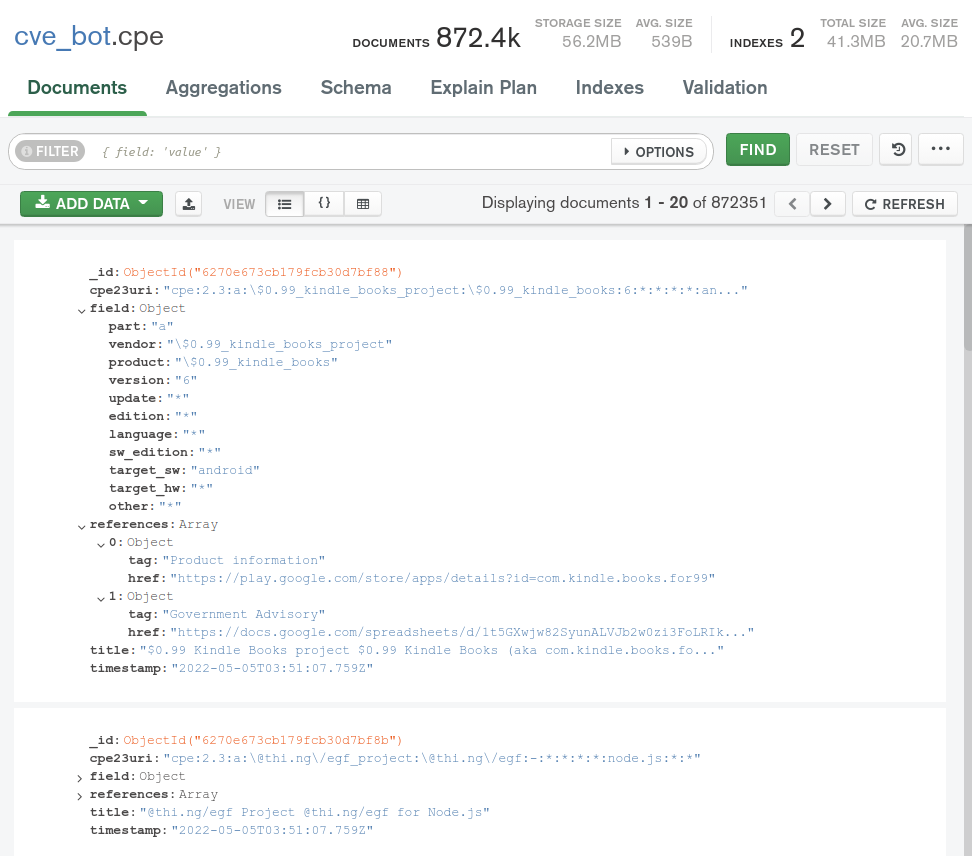
\includegraphics[width=0.45\textwidth]{pictures/DB_Cpe.png}
% 	}
% 	\quad %空格
% 	\subfloat[]{
% 		\label{pictures/DB_Cvedetails.png}
% 		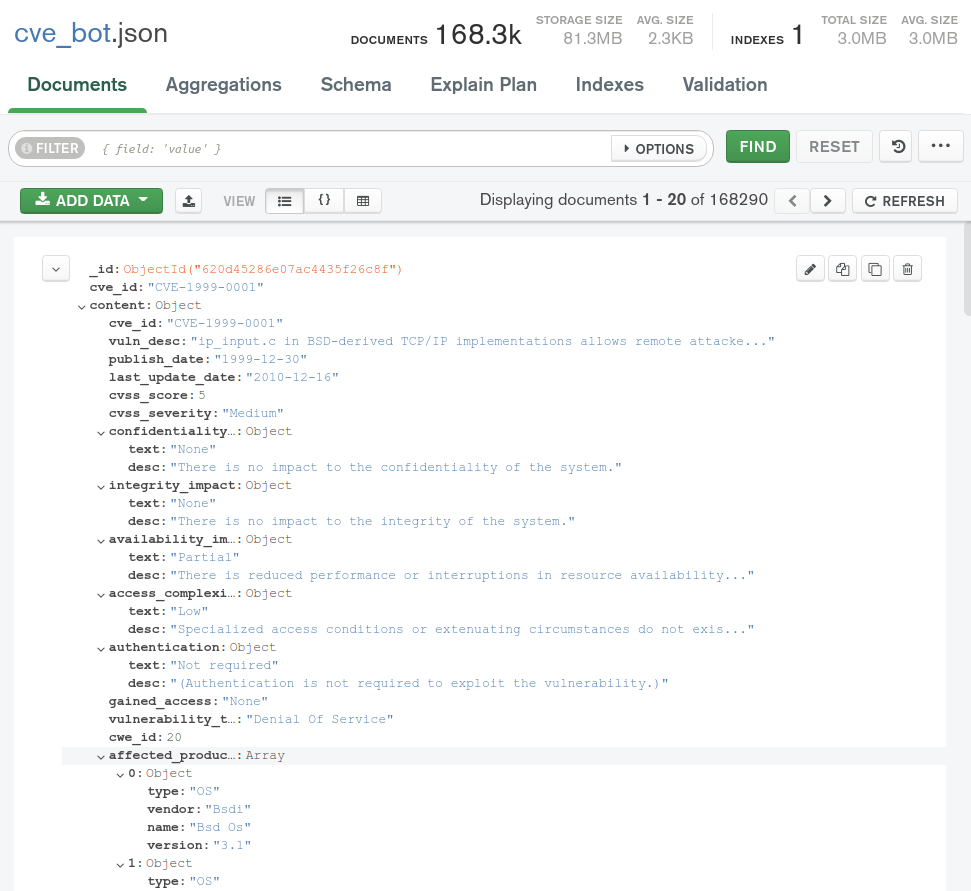
\includegraphics[width=0.45\textwidth]{pictures/DB_Cvedetails.png}
% 	}
% 	\\
% 	\subfloat[]{
% 		\label{pictures/DB_Cpe.png}
% 		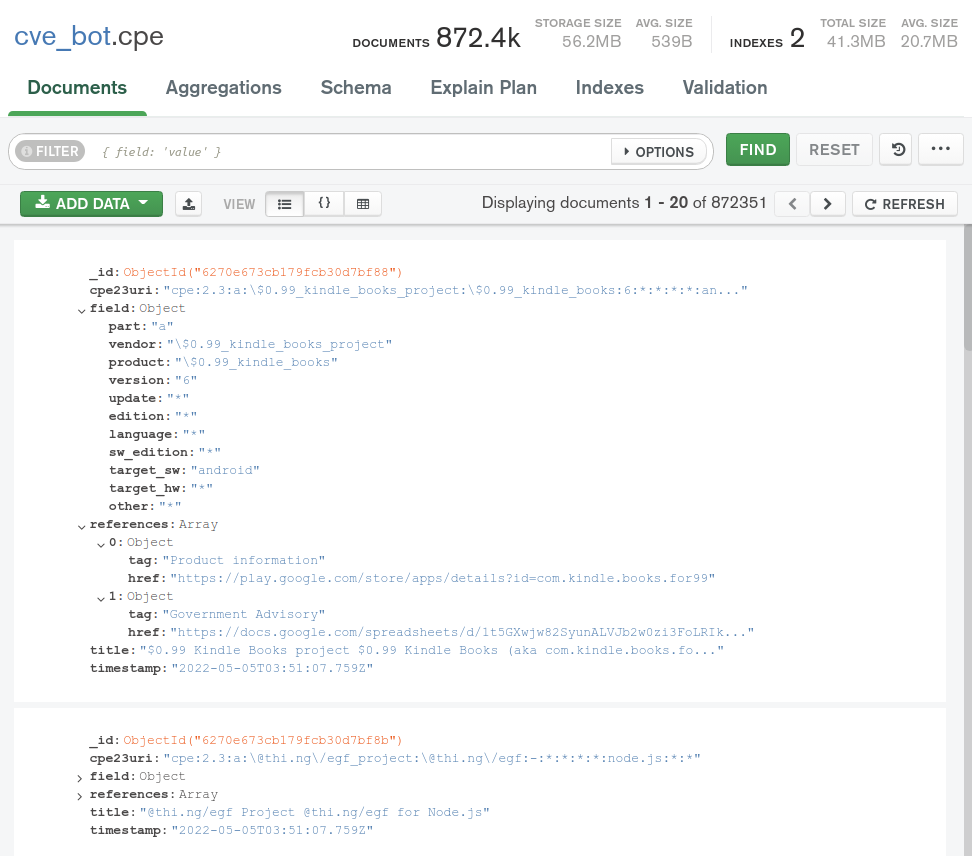
\includegraphics[width=0.45\textwidth]{pictures/DB_Cpe.png}
% 	}
% 	\quad
% 	\subfloat[]{
% 		\label{pictures/DB_Cpe.png}
% 		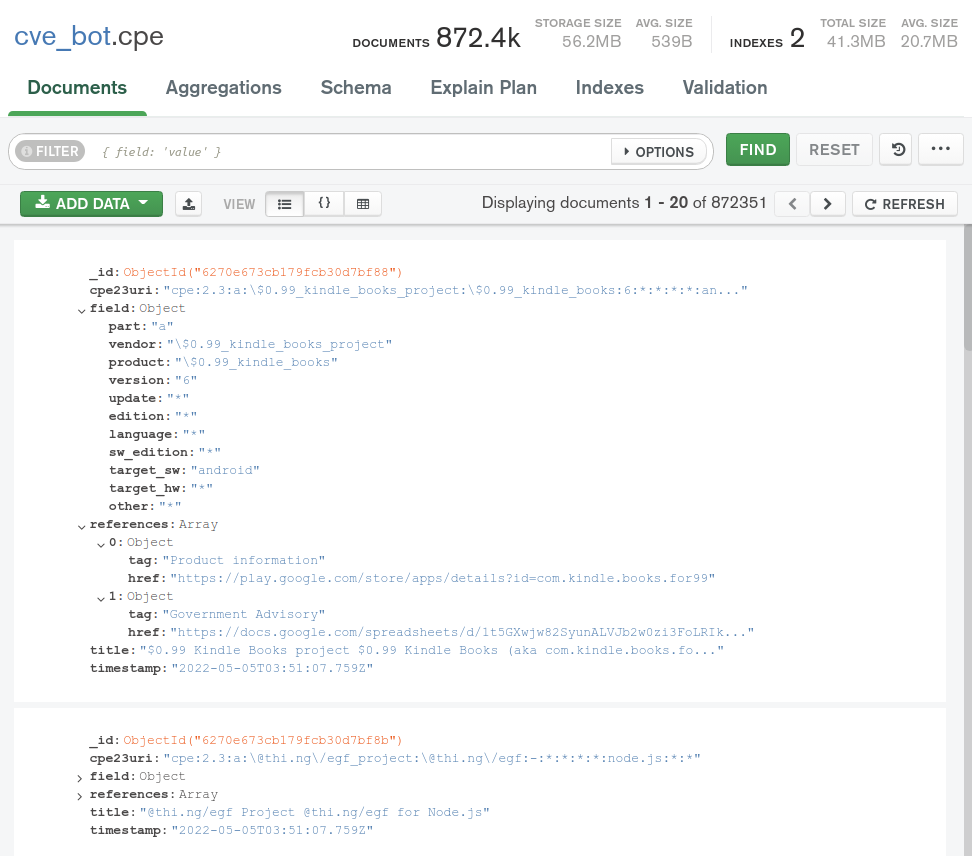
\includegraphics[width=0.45\textwidth]{pictures/DB_Cpe.png}
% 	}
% 	\caption{数据采集服务运行测试结果\\ \protect\subref{pictures/DB_Cpe.png} CPE 资产 JSON 数据,\protect\subref{pictures/DB_Cvedetails.png} cvedetails.com JSON 数据}
% 	\label{Fig:Crawl}
% \end{figure}

\section{知识图谱构建子系统测试}

\subsection{结点生成}

使用 Ray 库提供的 @ray.remote 装饰器与 ray.get() 方法,将全部漏洞数据根据并行度参数进行分割,开辟多进程对分块漏洞数据进行生成结点操作。

% 开辟 32 个进程生成漏洞结点、资产结点、资产家族结点、漏洞利用结点,总计约 120 万个结点。系统耗时约 5 分钟,如图\ref{pictures/Gen_Nodes.png}与图\ref{pictures/DB_Nodes.png}所示。
开辟 32 个进程并行生成漏洞结点、资产结点、资产家族结点、漏洞利用结点,总计约 120 万个结点。系统耗时约 5 分钟,如图\ref{pictures/Gen_Nodes.png}所示。

\buptfigure[width=\textwidth]{pictures/Gen_Nodes.png}{结点生成模块运行日志}{pictures/Gen_Nodes.png}

% \buptfigure[width=0.5\textwidth]{pictures/DB_Nodes.png}{数据库查询结点数量}{pictures/DB_Nodes.png}

\subsection{关系生成}

使用 Ray 库提供的 @ray.remote 装饰器与 ray.get() 方法,将全部漏洞数据根据并行度参数进行分割,开辟多进程对分块漏洞数据进行生成操作。

% 开辟 32 个进程生成``资产$-[$具有$]->$漏洞,漏洞$-[$影响$]->$资产;资产$-[$是子级$]->$资产家族,资产家族$-[$是父级$]->$资产;利用代码$-[$攻击$]->$资产,资产$-[$被攻击$]->$利用代码;利用代码$-[$利用$]->$漏洞,漏洞$-[$被利用$]->$漏洞代码''等关系,由于资产关系生成涉及正则匹配运算,无法有效利用数据库索引,且 CPU 性能消耗较大,因此生成时间较长。对总计约 120 万个结点共生成约 45 万条边(更多详细信息存储在边属性中),耗时约 1 小时 50 分钟,如图\ref{pictures/Gen_Rels.png}与图\ref{pictures/DB_Rels.png}所示。
开辟 32 个进程并行执行关系生成,由于资产关系生成涉及正则匹配运算,无法有效利用数据库索引,且 CPU 性能消耗较大,因此生成时间较长。对总计约 120 万个结点共生成约 45 万条边(更多详细信息存储在边属性中),耗时约 1 小时 50 分钟,如图\ref{pictures/Gen_Rels.png}所示。

\buptfigure[width=\textwidth]{pictures/Gen_Rels.png}{关系生成模块运行日志}{pictures/Gen_Rels.png}

% \buptfigure[width=\textwidth]{pictures/DB_Rels.png}{数据库查询关系数量}{pictures/DB_Rels.png}

\subsection{关系融合}

本系统设计上,结构化数据生成的漏洞实体具有 cve id 属性作为唯一标识;资产实体具有 cpe23uri 属性作为唯一标识;漏洞利用代码实体具有 edb-id 属性作为唯一标识。且在数据库控制器对象的方法中,使用 MERGE 等 CQL 子句保证不会向数据库插入重复的实体或属性。因此当前知识图谱内并不会出现语义相同的不同实体或关系。

关系融合模块作为适配使用深度学习模型进行命名实体识别结点生成与关系抽取方案的模块,当前仅在系统数据加工管线中留有接口,以备未来扩展需要。因此暂不作测试。

\section{持久化子系统与后端服务子系统测试}

\subsection{概览视图统计信息获取 /api/graph/}

% 向运行在 localhost 上的后端服务子系统发送 /api/graph/ 请求,获取当前知识图谱基础统计信息。后端返回各类资产数量统计、各类漏洞数量统计、各类代码利用数量统计等信息,如图\ref{pictures/Backend_api-graph-content.png}所示。
向运行在 localhost 上的后端服务子系统发送 /api/graph/ 请求,获取当前知识图谱基础统计信息。后端返回各类资产数量统计、各类漏洞数量统计、各类代码利用数量统计等信息,耗时约 200 毫秒,如图\ref{Fig:Backend_api_graph}所示。
% \buptfigure[width=0.45\textwidth]{pictures/Backend_api-graph-content.png}{/api/graph/ 请求响应数据}{pictures/Backend_api-graph-content.png}

% 耗时约 200 毫秒,如图\ref{pictures/Backend_api-graph.png}所示。

% \buptfigure[width=0.45\textwidth]{pictures/Backend_api-graph.png}{/api/graph/ 请求响应摘要}{pictures/Backend_api-graph.png}

\begin{figure}[!htbp]
	\centering
	\subfloat[]{
		\label{pictures/Backend_api-graph.png}
		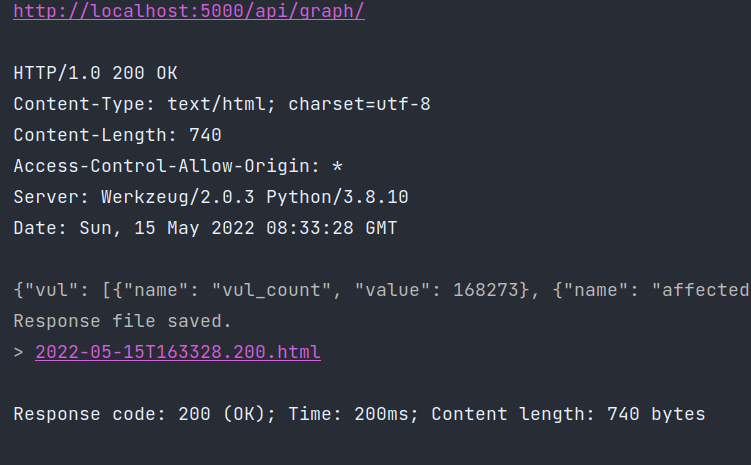
\includegraphics[width=0.46\textwidth]{pictures/Backend_api-graph.png}
	}
	\quad %空格
	\subfloat[]{
		\label{pictures/Backend_api-graph-content.png}
		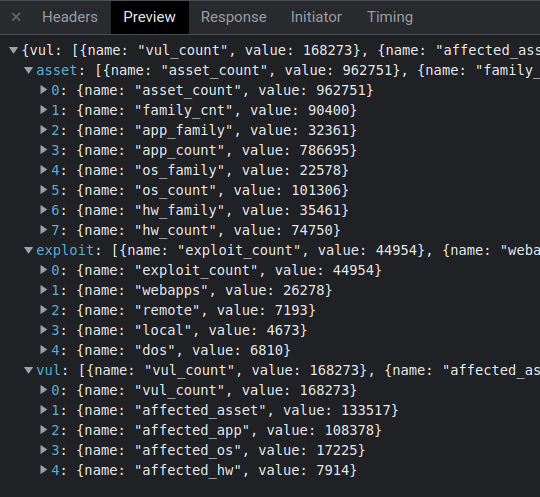
\includegraphics[width=0.46\textwidth]{pictures/Backend_api-graph-content.png}
	}
	\caption{统计信息获取 /api/graph/ 运行测试\\ \protect\subref{pictures/Backend_api-graph.png} 请求响应摘要,\protect\subref{pictures/Backend_api-graph-content.png} 请求响应数据}
	\label{Fig:Backend_api_graph}
\end{figure}

\subsection{可视化视图数据获取 /api/graph/<limit>}

% 向运行在 localhost 上的后端服务子系统发送 /api/graph/100 请求,获取当前知识图谱的 100 个漏洞结点以及与其相关的资产、利用代码结点、关系等信息,用于可视化。后端返回经绘图数据生成模块处理的绘图数据,包含分类、结点、关系三个数组,如图\ref{pictures/Backend_api-graph-100-content.png}所示。
向运行在 localhost 上的后端服务子系统发送 /api/graph/100 请求,获取当前知识图谱的 100 个漏洞结点以及与其相关的资产、利用代码结点、关系等信息,用于可视化。后端返回经绘图数据生成模块处理的绘图数据,包含分类、结点、关系三个数组,耗时约 640 毫秒,如图\ref{Fig:Backend_api_graph_100}所示。

% \buptfigure[height=0.4\textheight]{pictures/Backend_api-graph-100-content.png}{/api/graph/100 请求响应数据}{pictures/Backend_api-graph-100-content.png}

% 耗时约 640 毫秒,如图\ref{pictures/Backend_api-graph-100.png}所示。

% \buptfigure[height=0.4\textheight]{pictures/Backend_api-graph-100.png}{/api/graph/100 请求响应摘要}{pictures/Backend_api-graph-100.png}

\begin{figure}[!htbp]
	\centering
	\subfloat[]{
		\label{pictures/Backend_api-graph-100.png}
		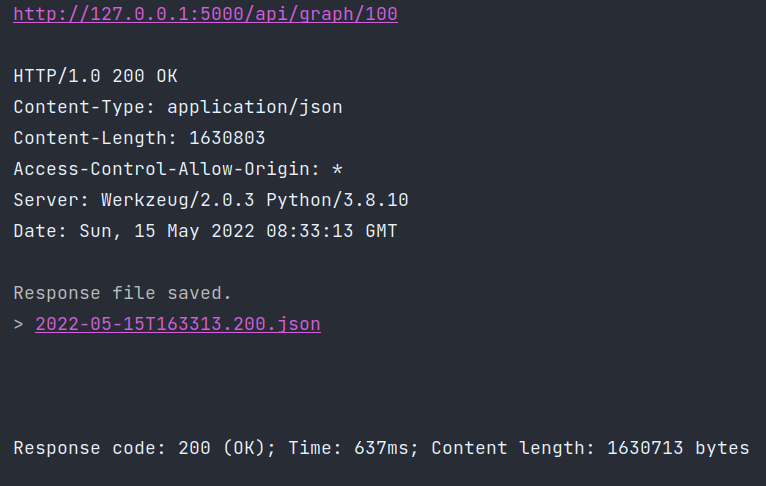
\includegraphics[width=0.46\textwidth]{pictures/Backend_api-graph-100.png}
	}
	\quad %空格
	\subfloat[]{
		\label{pictures/Backend_api-graph-100-content.png}
		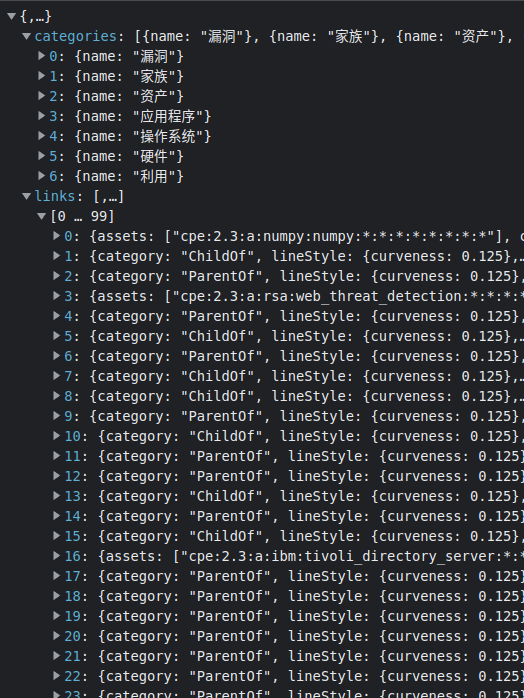
\includegraphics[width=0.46\textwidth]{pictures/Backend_api-graph-100-content.png}
	}
	\caption{可视化视图数据获取 /api/graph/100 运行测试\\ \protect\subref{pictures/Backend_api-graph-100.png} 请求响应摘要,\protect\subref{pictures/Backend_api-graph-100-content.png} 请求响应数据}
	\label{Fig:Backend_api_graph_100}
\end{figure}

\section{前端子系统测试}

\subsection{概览视图测试\label{概览视图测试}}

图\ref{pictures/Vis_Dashboard_Info.png}所示为概览视图。从 localhost 后端 /api/graph/ 端口加载数据,实际返回,根据瀑布流图可看出,通过刷新页面冷加载概览界面及各种网络请求耗时约 850ms,且加载过程中可视化图表有加载指示器提示正在加载、数据列表有默认数据``0''填充而非显示空白,用户体验较好。如图\ref{pictures/Vis_Dashboard_Waterfall.png}所示。

前端子系统全部界面均采用类 App 设计,具备响应式显示功能,卡片行列数可根据当前设备屏幕分辨率动态流式调整,保证在各种设备上均能正常显示。

\buptfigure[width=\textwidth]{pictures/Vis_Dashboard_Info.png}{概览视图预览}{pictures/Vis_Dashboard_Info.png}

\buptfigure[width=\textwidth]{pictures/Vis_Dashboard_Waterfall.png}{概览视图加载请求瀑布流}{pictures/Vis_Dashboard_Waterfall.png}

\subsection{可视化视图测试\label{可视化视图测试}}

图\ref{pictures/Vis_Full.png}所示为知识图谱概览。从 localhost 后端 /api/graph/30 端口加载数据,实际返回 1684 个结点、3368 条关系边,根据瀑布流图可看出,通过刷新页面冷加载可视化力引导图耗时约 1800ms,且加载过程中有加载指示器提示正在加载,用户体验较好。如图\ref{pictures/Vis_Waterfall.png}所示。

\buptfigure[width=\textwidth]{pictures/Vis_Full.png}{可视化视图概览}{pictures/Vis_Full.png}

\buptfigure[width=\textwidth]{pictures/Vis_Waterfall.png}{可视化视图加载请求瀑布流}{pictures/Vis_Waterfall.png}

图\ref{pictures/Vis_Full_New.png}所示为知识图谱细节图。力引导图为有向图,因此结点间的无向边使用两条有向边表示。图中蓝色结点为漏洞结点,绿色结点为资产家族结点,红色结点为受影响资产结点。可以看到,通过将漏洞所影响的大量资产关系替换成漏洞到资产家族的一个关系,大幅简化了图的结构,在使视觉观感清晰的同时,将鼠标移至漏洞至资产家族的边上可显示受该漏洞影响的所有资产,保证图谱数据的详细精确。

当鼠标移动至或触摸图中元素,包括各类结点和各类关系,会显示 Tooltip 指示,展现当前高亮元素的信息。点击结点或关系,将会弹出悬浮面板,展示结点或关系的更详细信息。

\buptfigure[width=\textwidth]{pictures/Vis_Full_New.png}{可视化视图 Tooltip 和弹出面板展示详细信息}{pictures/Vis_Full_New.png}

\subsection{搜索视图测试}

图\ref{pictures/Vis_Search.png}所示为搜索视图。搜索视图提供一个悬浮搜索框,允许用户对知识图谱进行精确查询。输入查询关键字并按下回车将发送异步 I/O 请求,后端服务将搜索整个知识图谱查找关键字相关信息,并将绘图数据返回前端。前端回调使用 ECharts 可视化库绘制力引导图展示数据。

\buptfigure[width=\textwidth]{pictures/Vis_Search.png}{搜索视图使用关键字搜索,呈现结点及关系}{pictures/Vis_Search.png}

% \subsection{控制台视图测试}

% 图\ref{pictures/Vis_Dashboard_Control.png}所示为控制台视图。
% \buptfigure[width=\textwidth]{pictures/Vis_Dashboard_Control.png}{关于视图}{pictures/Vis_Dashboard_Control.png}

\subsection{关于视图测试}

图\ref{pictures/Vis_About.png}所示为关于视图。关于视图清晰地展示了本系统名称、功能、作者、使用指南等信息。

\buptfigure[width=\textwidth]{pictures/Vis_About.png}{关于视图}{pictures/Vis_About.png}

\chapter{结束语}

\section{项目工作总结}

本文介绍了``基于漏洞知识图谱的可视化系统''的设计与实现。由于漏洞信息的收集与发布工作分散在互联网各处,且通常以纯文本的形式发布共享,这造成网络安全工作者及软硬件开发者,难以轻松直观地获知相关项目或资产的漏洞风险情况。而提供类似可视化漏洞知识图谱服务的多为商业公司、其系统不公开且收费高昂。

基于此背景,本文设计并实现了使用 GPL-3.0 自由软件许可证授权的``基于漏洞知识图谱的可视化系统'',全部代码在 \href{https://github.com/RiddMa/KnowledgeGraph-Visualization}{GitHub}\footnote{https://github.com/RiddMa/KnowledgeGraph-Visualization} 开源。其由数据采集子系统、知识图谱构建子系统、持久化子系统、后端服务子系统、前端子系统五部分组成。

针对五个子系统,本文第二章分别介绍了其相关技术调研与实现理论基础,分析并确定了开发本系统采用的技术栈,主要为:\lstinline|Python, Scrapy, MongoDB, Neo4j, Flask, HTML, CSS, JavaScript, Vue.js, Vuetify, ECharts|。

第三章针对系统数据流、功能和非功能需求进行了需求分析,细化系统开发目标。

第四章系统设计进行了系统概要设计、系统功能模块设计、系统详细设计:首先针对系统数据流分析,设计系统总体及分层结构,形成项目框架;随后划分功能模块、针对每个功能模块明确其功能与职责,并为模块绘制了类图与功能时序图。

第五章系统实现以流程图形式阐述各个子系统的设计与实现,以伪代码形式阐述关键功能模块的设计与实现。

第六章系统测试对系统运行速度与运行结果进行简单测试,以截图形式展示可视化系统的实现效果。

本系统具备并行数据采集能力、并行知识图谱构建能力、后端 API 及 Cron 风格定时控制能力、前端数据可视化展示与交互能力。能够在无人为干预情况下定时采集数据并更新知识图谱,且每次更新花费时间可以接受(爬虫时间依网络情况而定,小于一天;知识图谱更新时间约为两小时)。前端具备友好的响应式界面、清晰的图表展现知识图谱相关数据,通过力引导图实现的知识图谱可视化功能,允许用户拖拽、缩放、选中结点或关系弹出侧边栏显示详细数据。

\section{未来工作展望}

本系统借鉴微服务设计思想,将构建信息安全漏洞知识图谱任务分解成若干小任务的数据加工流。模块化设计使得系统具备强大的鲁棒性和扩展性。未来系统功能扩展主要在于智能化技术即各类机器学习及深度学习模型的引入方向。

针对数据采集子系统,未来可持续增加数据源,如 CNNVD、JVN 等;可借助搜索引擎,编写实现更智能的 Spider。例如,根据漏洞信息中提及的相关实体,使用搜索引擎获取搜索结果,对文本数据进行自动摘要提取信息主题,选择相关性较强的链接作为漏洞补充资料。或定期爬取技术博客、技术新闻等自然语言文本内容。

针对知识图谱构建子系统,使用深度学习模型进行命名实体识别、关系抽取、关系融合,实现实体语义去重与关系融合功能,将不同命名体系下的相同漏洞融合为同一实体。还可通过自然语言数据将部分未收录进 CPE 官方列表的资产、未被 CVE 等项目收录的漏洞作为补充加入知识图谱。

针对持久化子系统,随着知识图谱不断增大,Neo4j Community 单机版性能不足以支撑大数据量,可将知识图谱迁移至其他开源分布式图数据库如 Nebula Graph。由于本系统设计时尽量采用通用的 CQL 语句进行数据库操作而非使用 Neo4j 特定 ORM 对象,迁移工作可以较平滑进行。

针对后端服务子系统,为了应对未来可能增长的用户量,可以引入 Redis 内存数据库技术,引入 Celery 等消息队列技术,提高系统并发性能。同时,为了满足更多用户的需要,可以加入完善的用户系统,引入会话认证、权限管理等功能。为了方便管理员查看 APScheduler 服务运行状态,可在前端加入``控制台''视图,允许管理员手动控制后端微服务运行。

针对前端子系统,可以完善 UI 设计、增加更多可视化选项;优化移动端上的展示功能。

%%%%%%%%%%%%%%%%%%%%%%% Main Area ENDs Here %%%%%%%%%%%%%%%%%%%%%%%%
%\let\cleardoublepage=\cleardoublepagebak

\begin{nopagenumber}
	% Reference
	\clearpage\phantomsection\addcontentsline{toc}{chapter}{参考文献}
	\bibliographystyle{buptbachelor}
	\refbodyfont{\bibliography{ref}}

	% Thanks to page
	\clearpage
	\chapter{致\qquad{}谢}
	\normalsize\thankwords

\end{nopagenumber}

% 开题报告
% \blankmatter
% 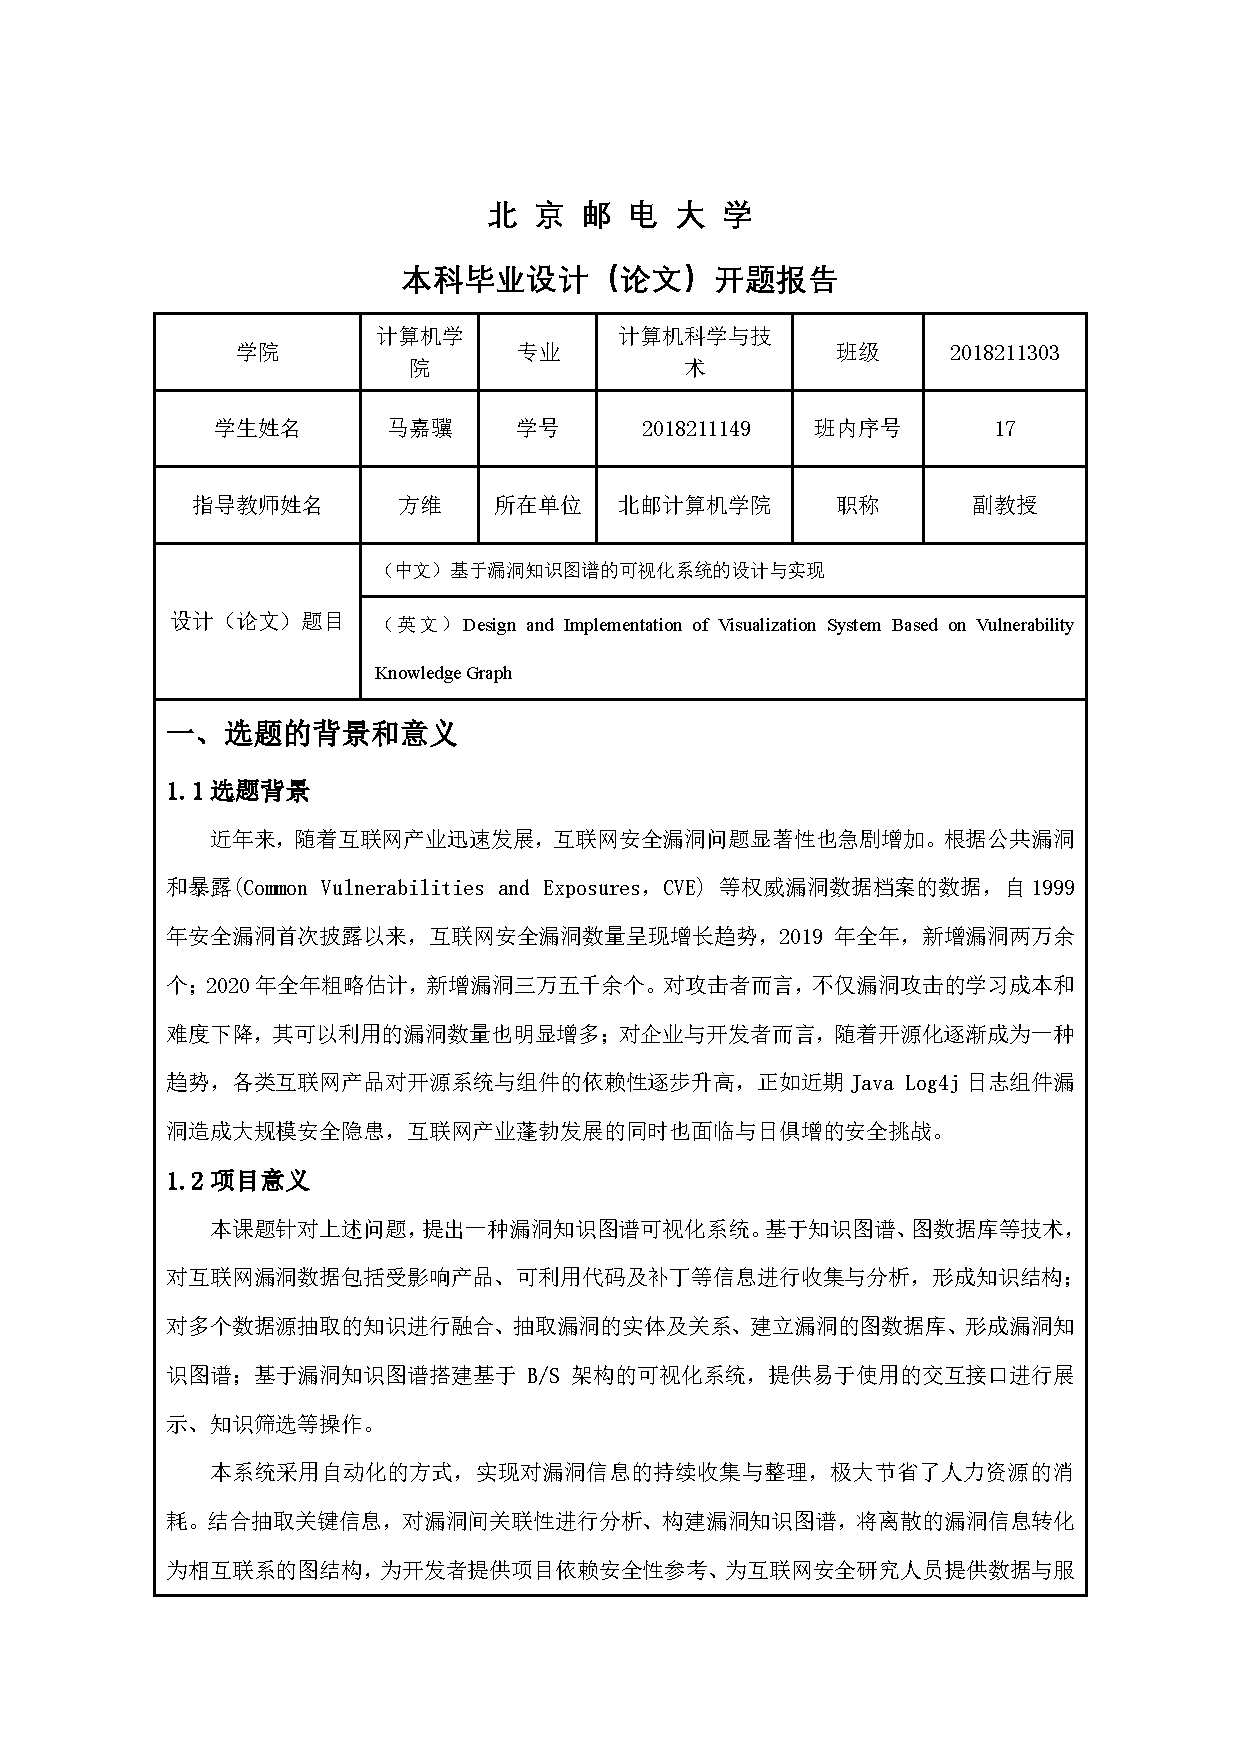
\includepdf[pages=-]{docs/openingReport.pdf}


% 中期检查表
% \blankmatter
% 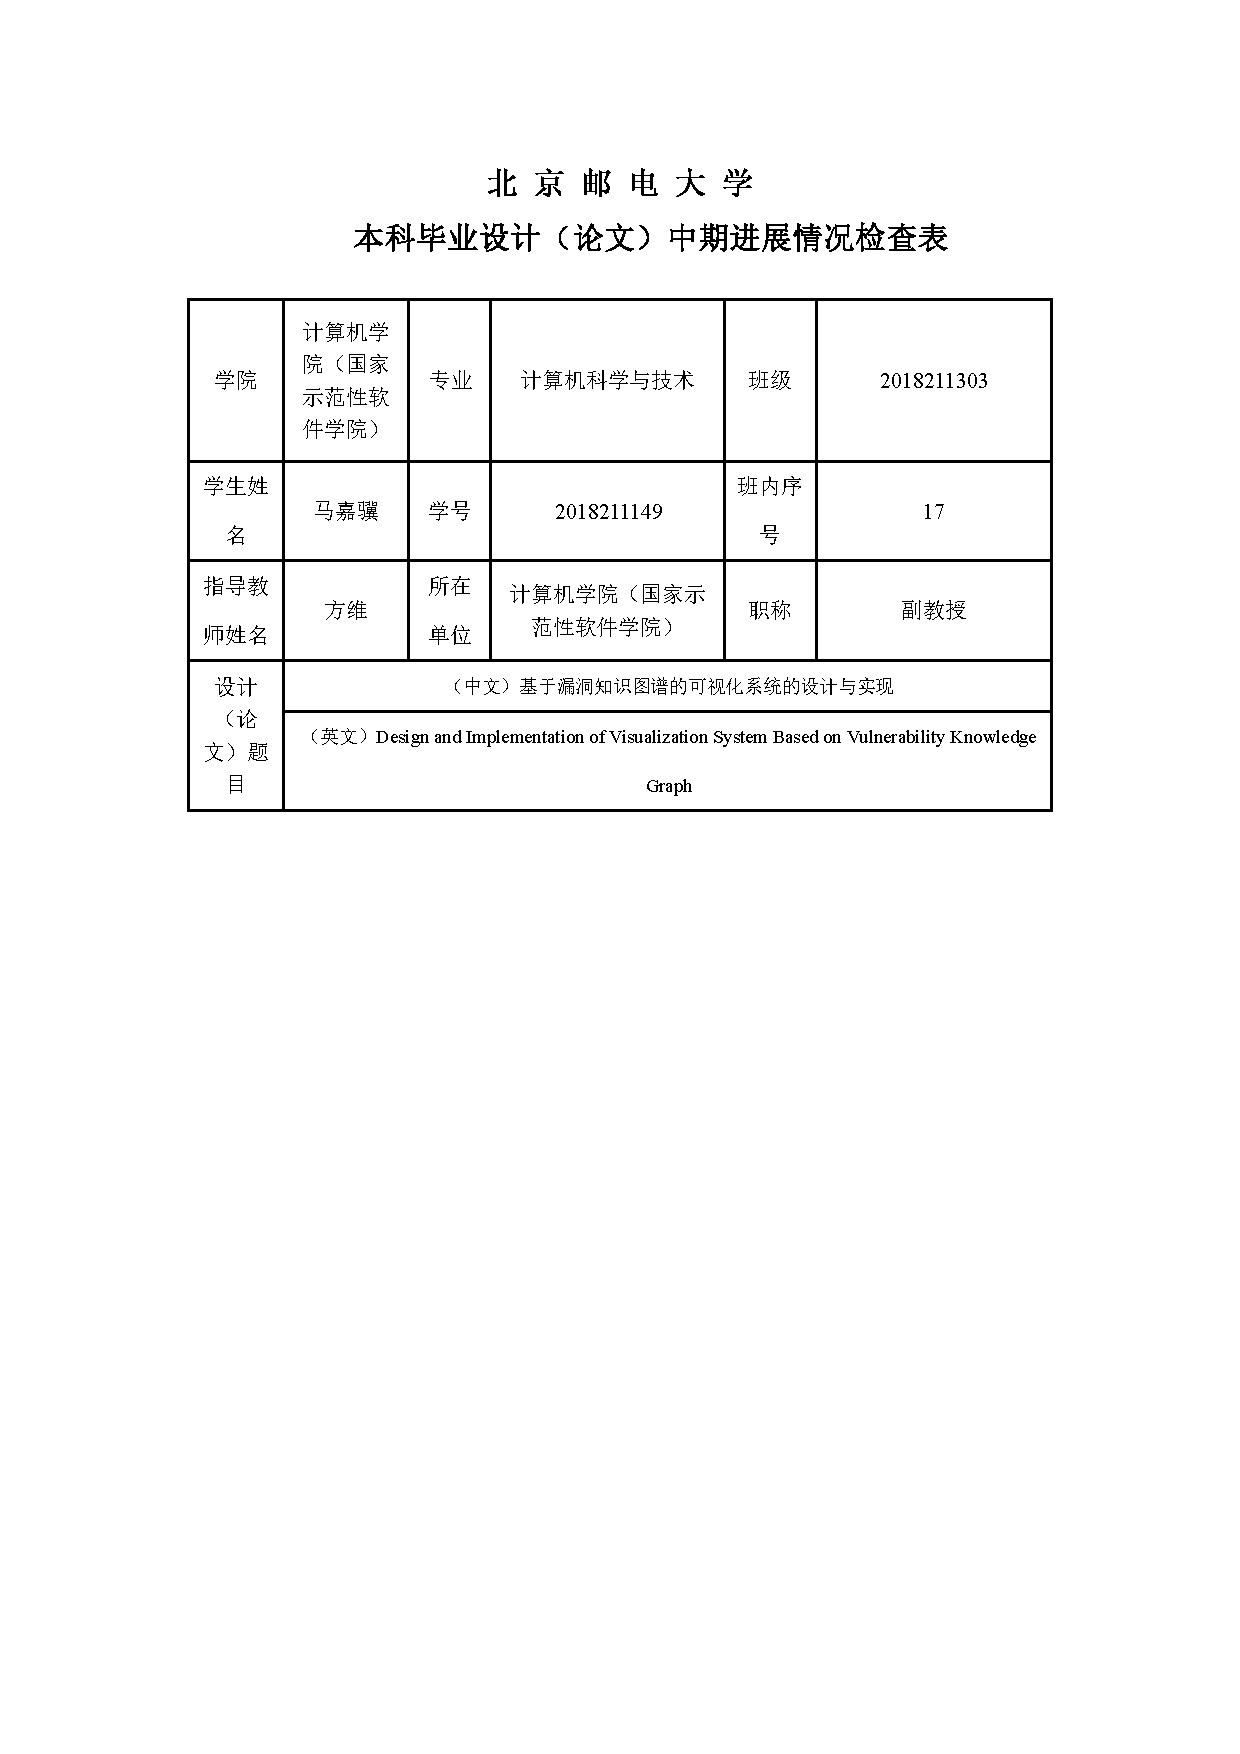
\includepdf[pages=-]{docs/interimReport.pdf}


\end{document}
